
\listfiles

\documentclass[12pt,a4paper]{article}

%در ورژن جدید زی‌پرشین برای تایپ متن‌های ریاضی، این سه بسته، حتماً باید فراخوانی شود
\usepackage{amsthm,amssymb,amsmath}

\usepackage{mathtools}
%دستوری برای وارد کردن واژه‌نامه انگلیسی به فارسی
\newcommand\persiangloss[2]{#1\dotfill\lr{#2}\\}
%%% ------- اضافه شده توسط نخ ------
%%% دستوری برای پنهان کردن چیزی از فهرست
\newcommand{\nocontentsline}[3]{}
\newcommand{\tocless}[2]{\bgroup\let\addcontentsline=\nocontentsline#1{#2}\egroup}
\usepackage[bottom]{footmisc}
\usepackage{indentfirst}
%\usepackage[english]{babel}
\usepackage{caption}
%\captionsetup[figure]{name=شکل}

%\captionsetup[contentsname]{name=فهرست}
%\renewcommand{\contentsname}{فهرست مطالب}

% ------ پایان تغییرات نخ
%بسته‌ای برای تنطیم حاشیه‌های بالا، پایین، چپ و راست صفحه
%\usepackage[top=50mm, bottom=50mm, left=50mm, right=50mm]{geometry}
%بسته‌ای برای نمایش تصاویر قرار داده شده در متن
\usepackage{graphicx}
\usepackage{subcaption}
\usepackage{array}
\usepackage{adjustbox}
\usepackage{tablefootnote}
\usepackage{amsfonts}
\usepackage{amssymb}
\usepackage{yfonts}

\usepackage[frak=boondox,bb=boondox,cal=boondoxo]{mathalfa}

\usepackage{xcolor,colortbl}
\definecolor{Gray}{gray}{0.90}
\definecolor{LGray}{gray}{0.95}

% بسته‌ و دستوراتی برای ایجاد لینک‌های رنگی با امکان جهش
\usepackage[pagebackref=false,colorlinks,linkcolor=blue,citecolor=magenta]{hyperref}
% چنانچه قصد پرینت گرفتن نوشته خود را دارید، خط بالا را غیرفعال و  از دستور زیر استفاده کنید چون در صورت استفاده از دستور زیر‌‌، 
% لینک‌ها به رنگ سیاه ظاهر خواهند شد و برای پرینت گرفتن، مناسب‌تر خواهد بود.
%\usepackage[pagebackref=false]{hyperref}
%بسته‌ای برای ظاهر شدن «مراجع»  در فهرست مطالب
\usepackage{tocbibind}
%\usepackage[Kashida]{xepersian}
%فراخوانی بسته زی‌پرشین و دستورات مربوط به نوع فونت‌ها
\usepackage{xepersian}
%\settextfont[Scale=1.1]{B Zar}

%\DefaultMathsDigits
%\DefaultMathsDigits

% وارد کردن دستور بالا الزامی نیست؛ چون در صورت وارد نکردن آن، فونت پیش‌فرض به صورت خودکار، فراخوانی می‌شود.
% چنانچه می‌خواهید که اعداد داخل فرمول‌ها، فارسی باشد، دستور زیر را فعال کنید
%\setdigitfont{Yas}
%%%%%%%%%%%%%%%%%%%%%%%%%%%%%%%%%%%%%%%%%%%%%%%%%%%
% تعریف قلم‌های فارسی و انگلیسی برای استفاده در بعضی از قسمت‌های متن
\defpersianfont\titr[Scale=1]{B Titr}
\defpersianfont\nastaliq[Scale=1.5]{IranNastaliq}
\defpersianfont\traffic[Scale=1]{B Traffic}
\defpersianfont\yekan[Scale=1]{B Yekan}
%اگر فونت‌های بالا را ندارید، دو خط بالا را غیر فعال و دو خط زیر را فعال کنید
%\defpersianfont\traffic[Scale=1]{XB Roya}
%\defpersianfont\yekan[Scale=1]{XB Kayhan}
%%%%%%%%%%%%%%%%%%%%%%%%%%%%%%%%%%%%%%%%%%%%%%%%%%%
% تعریف و نحوه ظاهر شدن قضایا، لم‌ها، تعریف‌ها و ...
\theoremstyle{definition}
\newtheorem{definition}{تعریف}[section]
\theoremstyle{theorem}
\newtheorem{theorem}[definition]{قضیه}
\newtheorem{lemma}[definition]{لم}
\newtheorem{proposition}[definition]{گزاره}
\newtheorem{corollary}[definition]{نتیجه}
\newtheorem{remark}[definition]{ملاحظه}
\theoremstyle{definition}
\newtheorem{example}[definition]{مثال}

\usepackage{zref-perpage}
\zmakeperpage{footnote}


%%%%%%%%%%%%%%%%%%%%%%%%%%%%%%%%%%%%%%%%%%%%%%%%%%%
\begin{document}
% دستوری جهت حذف کردن شماره صفحه و سربرگ، در صورت وجود (فقط در صفحه جاری)
\thispagestyle{empty}
\vspace*{-28mm}
% نحوه درج کردن لوگوی دانشگاه
\centerline{
\includegraphics[height=5cm]{logo.png}}

\begin{center}
%دستوری برای کم کردن فاصله بین لوگو و خط پایین آن
\vspace{-2mm}
{\large \titr
گروه مستقل مهندسی رباتیک
%دستوری برای تعیین فاصله بین دو خط
\\[2.1cm]
}

{\large \titr
گزارش تحقیقاتی درس هوش محاسباتی - الگوریتم‌های تکاملی
\\[2cm]
{\Large
الگوریتم‌ تکامل تفاضلی با تطبیق استراتژی برای بهینه‌سازی سراسری عددی
\\[2cm]
}

استاد درس:
\\[.5cm]
{\Large
دکتر نیک‌آبادی}
\\[1.5cm]
\large 
نام دانشجو:
\\[.5cm]
{\Large
نوید خزاعی}
\\[.5cm]
۹۲۱۳۵۰۰۸
\\[1.5cm]
}
%دستوری برای تعیین فاصله بین خطوط (نه دو خط) و تا وقتی که مقدار آن تغییر نکند، فاصله بین خطوط، همین مقدار است.
\baselineskip=1cm

{\large
اردیبهشت ۱۳۹۳
}
\end{center}

%دستوری برای رفتن به صفحه جدید
\newpage
\baselineskip=1cm

\baselineskip=.75cm
\newpage 
\pagenumbering{Alph}
\tocless {\section*}{چکیده}

تکامل تفاضلی یکی از روش‌های قدرتمند بهینه‌سازی در فضای پیوسته‌است که در آن برداری به نام بردار آزمایشی تولید می‌شود که استراتژی‌های تولید متفاوتی دارد و هر استراتژی نیز پارامترهایی دارد. برای پیدا کردن استراتژی مناسب و پارامترهای مناسب آن، جست‌وجوی کورکورانه و آزمون و خطا بسیار پرهزینه است. همچنین استراتژی‌ها و پارامترها ممکن است در مراحل مختلف تکامل متفاوت باشند. در مقاله‌ی انتخابی ما روشی به نام تکامل تفاضلی خودتطبیقی ارایه شده‌است که این مشکلات را تا حدی حل می‌کند و استراتژی‌ها بر اساس احتمال تولید بردارهای امیدبخش برای ورود به نسل بعد، که در طول تکامل یادگرفته می‌شود، از استخر استراتژی‌ها انتخاب می‌شوند. آزمایش‌ها با ۲۶ تابع آزمون معروف در تکامل تفاضلی انجام شده‌اند و با ۸ روش معمول مقایسه انجام شده‌است. برای درک بهتر ادبیات مساله، کارهای مرتبط را فراتر از آن‌چه در مقاله آورده شده‌بود بیان کردیم و جدول‌هایی را برای این منظور طراحی نمودیم. تحلیل‌هایی نیز از نتایج گرفته‌شده ارایه خواهد شد.


\newpage
\tocless\tableofcontents
\newpage 
\pagenumbering{arabic}
\section{مقدمه}
الگوریتم‌های تکاملی، الگوریتم‌هایی هستند که از تکامل طبیعی موجودات الهام گرفته‌ شده‌اند و در حل مسایل بهینه‌سازی، در زمینه‌های بسیار متنوعی، موفق بوده‌اند. اما در عمل، برای رسیدن به یک پیاده‌سازی کارا در مساله‌ی واقعی، نیاز است استراتژی‌های مناسب برای انتخاب عملگر‌های تکاملی انتخاب شوند و علاوه‌ بر آن، باید مقادیر مناسب برای پارامترهای هر استراتژی نیز به‌دست‌آید. انجام این انتخاب‌ها با روش‌های آزمون و خطا، می‌تواند بسیار وقت‌گیر باشد. به همین دلیل، پژوهش‌های بسیاری بر روی تطبیق عملگرها و پارامترهای الگوریتم‌های تکاملی انجام شده‌است.

برای بررسی بهتر روش‌های تطبیق، دسته‌بندی‌های گوناگونی ارایه شده‌است که از جمله‌ی آن‌ها می‌توان به موردی که در \cite{category} آورده‌ شده‌است، اشاره کرد. در این دسته‌بندی، روش‌های تطبیق به دو دسته‌ی مطلق\LTRfootnote{ Absolute} و تجربی\LTRfootnote{ Empirical} تقسیم می‌شوند. روش‌های مطلق، چگونگی تغییرات پارامترها را از قبل مشخص می‌کنند. این در حالی است که روش‌های تجربی، قوانین تنظیم پارامترها را با توجه به اصل رقابت در الگوریتم‌های تکاملی، به‌روز‌رسانی می‌کنند. از طرفی، روش‌های تنظیم پارامتر در الگوریتم‌های تکاملی به سه گونه تقسیم می‌شوند \cite{adapt-category} : 


\begin{itemize}
\renewcommand{\labelitemi}{$\bullet$}

\item \textbf{قطعی\LTRfootnote{ Deterministic} :‌ }
قوانین مطلق، که بر اساس مجموعه‌ای از استدلال‌های منطقی در زمینه‌ی حلِ مساله‌ی مورد نظر به‌دست آمده‌اند، چگونگی تغییرات پارامترها را مشخص می‌کنند و هیچ بازخوردی از پروسه‌ی جست‌وجو نمی‌گیرند. 

\item \textbf{تطبیقی\LTRfootnote{ Adaptive} : }در این روش، پارامترها با توجه به بازخوردی که از پروسه‌ی جست‌وجو گرفته‌‌می‌شود، تنظیم می‌شوند.

\item \textbf{خود تطبیقی\LTRfootnote{ Self-Adaptive} : }
 
پارامترها در درون خود افراد جامعه قرار داده‌می‌شوند و روال تکامل با درنظرگرفتن پارامترها در جواب‌های مساله انجام می‌گیرد. به این ترتیب که پارامترهایی که جواب‌های بهتری تولید کنند، به بقا ادامه می‌دهند.
\end{itemize}


الگوریتم تکامل تفاضلی  که در سال ۱۹۹۷ ارایه شد \cite{DE}، روشی ساده و در عین حال قدرتمند برای جست‌وجو در فضای پیوسته است. این روش مبتنی بر جمعیت است و یک جست‌وجوی تصادفی به شمار می‌آید. این الگوریتم در زمینه‌های زیادی به کارگرفته شده و نتایج موفقیت‌آمیزی از خود نشان‌ داده‌است. در این الگوریتم که در بخش آتی به بررسی جزییات آن خواهیم پرداخت، استراتژی‌های زیادی برای تولید برداری به نام بردار آزمایشی\LTRfootnote{ Trial vector} وجود دارد که ممکن است تنها برخی از آن‌ها در حل یک مساله‌ی خاص، کارا باشند. از طرفی، سه پارامتر مهم در تکامل تفاضلی وجود دارند که مقادیر آن‌ها تاثیر چشم‌گیری بر کارایی الگوریتم دارد. این سه پارامتر عبارت‌اند از تعداد جمعیت 
$\mathit{NP}$، 
ضریب مقیاس
$\mathit{F}$،
و نرخ بازترکیبی
$\mathit{CR}$.


انتخاب استراتژی مناسب برای تولید بردار آزمایشی و تنظیم پارامتر‌های یاد شده به روش سعی‌وخطا، هزینه‌بر و زمان‌گیر است. علاوه بر آن در حین اجرای الگوریتم، با حرکت در فضای جست‌وجو و جابه‌جا شدن میان نواحی مختلف، ممکن است استراتژی متفاوتی برای کارایی در آن‌ ناحیه نیاز باشد و یا مقادیر بهینه‌ی پارامترها تغییر کند. به همین‌ دلیل بهتر است استراتژی انتخاب بردار آزمایشی و مقادیر پارامترها در حین تکامل به صورت تطبیقی تنظیم شوند. در مقاله‌ی انتخاب‌شده، یک روش خودتطبیقی برای انتخاب بهترین استراتژی انتخاب بردار آزمایشی و مقادیر پارامترهای مناسب آن ارایه شده‌است. در روش ارایه‌شده، خودتطبیقی به وسیله‌ی یادگیری از تجربه‌ی قبلی در تولید جواب‌های امیدبخش انجام می‌شود.

در هر نسل، مجموعه‌ای از استراتژی‌های انتخاب به همراه مقادیر پارامترهای نسبت‌‌ داده‌شده به آن‌ها، به صورت جداگانه به افراد مختلف جمعیت فعلی اعمال خواهد شد و این انتخاب، با توجه به احتمال‌های یادگرفته‌شده در نسل‌های قبل انجام می‌شود. 

در ادامه‌ی این گزارش، در بخش ۲ به معرفی الگوریتم تفاضل تکاملی می‌پردازیم. در بخش ۳ مروری بر کارهای مرتبط آورده‌ شده‌است. در بخش ۴ الگوریتم خودتطبیقی تفاضل تکاملی\LTRfootnote{ SaDE} ارایه شده‌است و در بخش ۵ ارزیابی آن آورده شده‌است. در پایان، در بخش ۶ به نتیجه‌گیری از مقاله‌ی بررسی‌شده خواهیم پرداخت.


\newpage
\section{تکامل تفاضلی}
\subsection{جمعیت و افراد}
در تکامل تفاضلی، یک جمعیت
$\mathit{NP}$تایی
از بردار پارامترهای
$\mathit{D}$
بُعدی داریم که افراد جمعیت ما در نسلِ
$\mathit{G}$
هستند که راه‌حل به سمت بهینه‌ی سراسری را در خود دارند، مانند:‌
\begin{equation}
\label{de-individual}
{\bf{X}}_{i,G} =  \lbrace {x_{i,G}^{1} , \dots , x_{i,G}^{D} } \rbrace , i=1, \dots , \mathit{NP} 
\end{equation}

بهتر است جمعیت اولیه تا حد امکان تمام فضای جست‌وجو را به صورت یکنواخت پوشش دهد و این مقداردهی، به صورت تصادفی و با مشخص کردن مقادیر کمینه و بیشینه‌ای برای هر پارامتر، انجام شود که نمونه‌ی آن در فرمول شماره‌ی 
(۱)
مقاله‌ی مورد نظر\cite{Sade}، آورده‌ شده‌است.

\subsection{عمل جهش}

پس از تولید جمعیت اولیه، یک بردار جهش
\( {\bf{V}}_{i,G} \)
برای هر فرد 
\( {\bf{X}}_{i,G} \)،
 که بردار هدف نامیده می‌شود، تولید می‌شود. این بردار که به شکل 
\( { {\bf{V}}_{i,G} =  \lbrace {v_{i,G}^{1} , \dots , v_{i,G}^{D} } \rbrace } \)
است، با استراتژی‌های متفاوتی محاسبه می‌شود، برای نمونه می‌توان به پنج نمونه‌ی پیاده‌سازی‌شده\RTLfootnote{ پیاده‌سازی‌ این استراتژی‌ها در آدرس 
\lr{http://www1.icsi.berkeley.edu/\~storn/code.html} 
 برای استفاده‌ی عمومی در دسترس است.} از این استراتژی‌ها اشاره کرد: 
\begin{enumerate}
\item {\lr{DE/rand/1}} : 
\vspace{-0.2cm}
\begin{equation}
{\bf{V}}_{i,G} = {\bf{X}}_{r_{1}^i , G} + F \cdot ( {\bf{X}}_{r_{2}^i , G} - {\bf{X}}_{r_{3}^i , G} ) 
\end{equation}

\item {\lr{DE/best/1}} : 
\vspace{-0.2cm}
\begin{equation}
{\bf{V}}_{i,G} = {\bf{X}}_{best , G} + F \cdot ( {\bf{X}}_{r_{1}^i , G} - {\bf{X}}_{r_{2}^i , G} ) 
\end{equation}

\item {\lr{DE/rand-to-best/1}} : 
\vspace{-0.2cm}
\begin{equation}
{\bf{V}}_{i,G} = {\bf{X}}_{i , G} + F \cdot ( {\bf{X}}_{best , G} - {\bf{X}}_{i , G} ) +  F \cdot ( {\bf{X}}_{r_{1}^i , G} - {\bf{X}}_{r_{2}^i , G} ) 
\end{equation}

\item {\lr{DE/best/2}} : 
\vspace{-0.2cm}
\begin{equation}
{\bf{V}}_{i,G} = {\bf{X}}_{best , G} +  F \cdot ( {\bf{X}}_{r_{1}^i , G} - {\bf{X}}_{r_{2}^i , G} )  +  F \cdot ( {\bf{X}}_{r_{3}^i , G} - {\bf{X}}_{r_{4}^i , G} ) 
\end{equation}
\vspace{0.1cm}

\item {\lr{DE/rand/2}} : 
\begin{equation}
{\bf{V}}_{i,G} = {\bf{X}}_{r_{1}^i , G} +  F \cdot ( {\bf{X}}_{r_{2}^i , G} - {\bf{X}}_{r_{3}^i , G} )  +  F \cdot ( {\bf{X}}_{r_{4}^i , G} - {\bf{X}}_{r_{5}^i , G} ) 
\end{equation}

\end{enumerate}

اندیس‌های 
\( r_{1}^i , r_{2}^i , r_{3}^i , r_{4}^i , r_{5}^i \)
 اعداد طبیعی منحصر به فردی هستند که به صورت تصادفی در بازه‌ی 
 \( [1,\mathit{NP}] \)
 تولید می‌شوند که از اندیس 
 $\mathit{i}$
 نیز متفاوت هستند. این اندیس‌ها برای هر بردار جهش تنها یک‌بار تولید می‌شوند. ضریب مقیاس\LTRfootnote{ Scaling factor} 
 $\mathit{F}$
 نیز یک پارامتر کنترلی مثبت است که تاثیر بردار تفاضل را کنترل می‌کند. بردار 
 \( {\bf{X}}_{best, G} \)
 نیز بهترین فرد موجود در نسل
  \( G \) 
  است.   
  
\subsection{عمل بازترکیبی}

پس از فاز جهش، عملگر بازترکیبی به هر جفت بردار‌های هدف 
\( {\bf{X}}_{i,G} \)
و جهش 
\( {\bf{V}}_{i,G} \)
نظیر آن اعمال می‌شود تا بردار آموزشی 
\( {\bf{U}}_{i,G} = (u_{i,G}^1, u_{i,G}^2, \dots , u_{i,G}^D ) \)
ساخته‌شود. در نسخه‌ی پایه‌ی تکامل تفاضلی، بازترکیبی دو جمله‌ای (یک‌نواخت) به این شکل تعریف می‌شود:

\begin{equation}
\label{binomial}
u_{i,G}^j =
  \begin{cases}
   v_{i,G}^j , & \text{\lr{if }} (rand_j[0,1) \le \mathit{CR} ) \text{\lr{ or }} (j=j_{rand}) \\
   x_{i,G}^j , & \text{\lr{otherwise}}
  \end{cases}
  \hspace{0.2cm} , j = 1,2, \dots , D.
\end{equation}

در فرمول 
\ref{binomial}
نرخ بازترکیبی 
\( \mathit{CR} \) 
توسط کاربر در بازه‌ی 
$ [ 0 ,1 ) $ 
تعریف می‌شود که کسری از پارامترهایی را که باید از بردار جهش کپی شوند، مشخص می‌کند. 
$ j_{rand} $ 
یک عدد تصادفی در بازه‌ی 
$[ 1 , D ] $
است. عملگر بازترکیبی دیگری نیز وجود دارد که در آن، پارامترهای بردار آموزشی از نقطه‌ای تصادفی با پارامترهای بردار جهش جایگزین می‌شوند،‌ تا وقتی که برای اولین بار 
$rand_j [0,1) > \mathit{CR}$
شود. پارامترهای باقی‌مانده نیز از بردار هدف به ارث برده می‌شوند. دقت کنید که شرط 
$j=j_{rand}$ 
نیز قرارداده شده‌است تا بردار آزمایشی تولید شده، دست کم در یک پارامتر با بردار هدف تفاوت داشته باشد. این عملگر شبیه عمل‌گر بازترکیبی حلقوی دو نقطه‌ای است. 

\subsection{عمل انتخاب} 
اگر پارامتر‌های یک بردار آزمایشی از محدوده‌های کمینه و بیشینه‌ی نظیر خود خارج شوند،‌ با توزیعی یکنواخت، مقداری تصادفی در بازه‌ای از پیش‌ تعیین‌شده انتخاب شده و جاگذاری می‌شود. پس از آن، مقدار تابع ارزیابی برای همه‌ی بردارهای آموزشی محاسبه می‌شود و عملگر انتخاب اعمال می‌شود؛ به این ترتیب که مقدار تابع ارزیابی برای هر بردار آزمایشی 
$f({\bf{U}}_{i,G})$
با مقدار تابع ارزیابی برای بردار هدف نظیر آن 
$f({\bf{X}}_{i,G})$
مقایسه می‌شود، در صورتی که این مقدار برای بردار آزمایشی کمتر یا مساوی مقدار بردار هدف باشد، بردار هدف در جمعیت با بردار آزمایشی نظیرش جاگزین می‌شود و به نسل بعد می‌رود؛ در غیر این صورت خودش در جمعیت باقی‌ می‌ماند و در نسل بعد نیز ظاهر می‌شود. 

عملگر انتخاب را می‌توان به این شکل نشان‌داد: 

\begin{equation}
{\bf{X}}_{i, {G+1} } =
  \begin{cases}
   {\bf{U}}_{i,G} , & \text{\lr{if }} f({\bf{U}}_{i,G}) \le f({\bf{X}}_{i,G}) \\
   {\bf{X}}_{i,G} , & \text{\lr{otherwise}}
  \end{cases}
\end{equation}

الگوریتم
\lr{DE}
در جدول ۱ مقاله‌ی مورد نظر آورده شده‌است که در آن نسل اولیه تولید می‌شود و سپس تا رسیدن به یک شرط خاتمه، سه مرحله‌ی جهش، بازترکیبی و انتخاب تکرار می‌شود. 


%Should be redsigned, quality is awful 
%\makebox[\textwidth]{%
%\begin{tabular}{@{}cc@{}}
%\frame{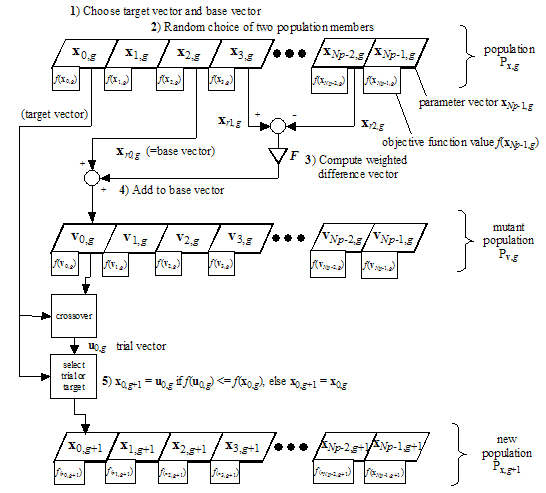
\includegraphics[width=80mm]{de2.jpg}} 
%\\
%\small  \textbf{دی ای به روایت تصویر؟:دی}
%\end{tabular}}
 


%جاگذاری جدول ۱ //TODO

\newpage
\section{کارهای مرتبط}
\label{sec:related}
کارایی الگوریتم 
\lr{DE}
معمول، به شدت به استراتژی تولید بردار آزمایشی و مقدار پارامترهای مورد استفاده بستگی دارد. انتخاب نامناسب استراتژی یا مقادیر پارامترها ممکن است منجر به همگرایی زودرس و یا سکون\LTRfootnote{ Stagnation} شود که اثبات آن به طور مفصل در 
\cite{demon1} , \cite{demon2} , \cite{demon3} , \cite{demon4}
 و 
 \cite{demon5} 
 آورده شده‌است. (متاسفانه مقاله‌ی مورد نظر در نوشتن این پاراگراف نه تنها ترتیب عددی ارجاعات را حفظ نکرده‌است بلکه آشکارا قالب ارجاع را نیز برهم زده‌است!).
 
از آن‌جا که مقاله‌ی مورد نظر از بررسی این اثبات‌ها عبور کرده‌است، نگاهی مختصر بر این مراجع داشتیم، که البته کتاب \cite{demon1} در دسترس نبود. در \cite{demon2} ابتدا مثالی از اجرای الگوریتم که به سکون منجر می‌شود آورده شده‌است، سپس به بررسی علل این سکون پرداخته‌است و با تعمیم نقش متغیرها در حالت کلی‌تر اجرای الگوریتم، و تاثیر آن‌ها در مشخص‌کردن فضای جست‌وجوی ممکن، تحلیل‌هایی ارایه شده‌است. همچنین اثبات شده‌است که در رابطه‌ی بازترکیبی خاص استفاده‌شده در آن مقاله، تنها تعداد مشخصی از بردارهای آزمایشی قابل تولید هستند که به نظر می‌رسد با روشی مشابه می‌توان هر رابطه‌ی بازترکیبی دیگر مانند \ref{binomial} را بررسی نمود. در نتیجه‌ی تولید بردارهای آزمایشی محدود، اگر هیچ‌کدام از آن‌ها نتوانند به‌جای بردار هدف متناظر در جمعیت جای‌گزین شوند، سکون رخ می‌دهد. همچنین مقادیری برای پارامترها در این مقاله پیشنهاد شده‌است.

  در \cite{demon3} الگوریتم بر روی چند تابع تست تک‌قله‌ای و چند قله‌ای اجرا شده‌است و با دو نمونه از الگوریتم استراتژی تکاملی مقایسه‌ شده‌است و بیشتر از آن‌که اثبات خاصی آورده شده‌باشد، از استدلال‌های شهودی و مشخص کمک‌گرفته شده‌است و در انتها، با مقایسه‌ی سه الگوریتم، به این نتیجه می‌رسد که حساسیت \lr{DE} نسبت به تغییرات در پارامترها بسیار بیشتر است. 
  
  در \cite{demon4} آورده شده‌است که می‌توان با کنترل تنوع جمعیت، تعادلی را میان اکتشاف و استخراج ایجاد نمود و در نتیجه از سکون و همگرایی زودرس جلوگیری کرد. با توجه به نقش پارامترها در کارایی الگوریتم، یک روش تطبیقی برای \lr{DE} ارایه شده‌است که مبتنی بر ایده‌ی کنترل تنوع جمعیت است و روابط کنترلی در آن با استفاده از پارامترهای الگوریتم و پارامترهای معرفی‌شده استخراج شده‌است. با بدست آوردن واریانس مورد انتظار جمعیت پس از بازترکیبی، و نوشتن این رابطه برای دو نسل متوالی و بررسی نسبت آن‌ها، به یک پارامتر کنترلی رسیده‌است که تاثیر آن برروی همگرایی و سکون را تحلیل کرده و مقادیری را برای آن یشنهاد داده‌است. همچنین تحلیلی بر روی یک نسخه‌ی چند جمعیتی از روش تطبیقیِ ارایه‌شده نیز انجام شده‌است. 
  
  در \cite{demon5} تلاش‌ شده‌است تا با تغییر ضریب مقیاس، بهبود ایجاد شود. دو حالت انتخاب تصادفی و انتخاب متناسب با زمان برای این پارامتر بررسی شده‌است و نتیجه‌ با 
  \lr{DE}
  معمول، 
  \lr{PSO}\cite{pso}،
  \lr{PSO-TVIW}\cite{pso-tviw}
  و 
    \lr{PSO-RANDIW}\cite{pso-randiw}
    در هفت تابع ‌آزمون پرکاربرد مقایسه شده‌است، این کار هیچ‌گونه تحلیل ریاضی قابل قبولی بر روی پیشرفت‌های حاصل‌شده انجام نداده‌است.
    
    ابتدایی‌ترین کارها در زمینه‌ی انتخاب استراتژی و تعیین پارامترهای آن، که همگی راه‌کارهایی تجربی را به دست‌می‌دهند، در جدول 
    \ref{tabold}
    آورده‌ شده‌اند. 


\renewcommand{\arraystretch}{2}

\begin{table}[h!]

\caption{روش‌های تجربی تنظیم استراتژی و پارامترها\textsuperscript{*}}
\centering
\begin{adjustbox}{center}

\begin{tabular}{ | c | >{\centering}m{0.3\textwidth} | >{\centering}m{0.22\textwidth} | m{0.55\textwidth}| }

\hline

%inserts double horizontal lines
مرجع &
موارد بررسی‌شده & 
 مقادیر پیشنهادی & 
\multicolumn{1}{c|}{توضیحات}
\tabularnewline [0.5ex]
\hline
% inserts single horizontal line
\cite{15} & 
%\parbox[t]{5cm}{
$\mathit{NP},\mathit{CR},\mathit{F}$

مقایسه‌ با 
\lr{ASA}\footnotemark[1]
و
\lr{ANM}\footnotemark[2]
%} %end of parbox
& 
$\mathit{NP} \in [ 5D,10D ]$

$\mathit{CR_{init}} = 0.5 $

$\mathit{F_{init}} = 0.5 $

$\mathit{F_{eff}} \in [0.4 , 1 ] $ 
& 
$\mathit{CR_{init}} = 0.9 $
برای تک‌قله‌ای و یا همگرایی زودرس مطلوب.

افزایش 
$\mathit{F}$
یا 
$\mathit{NP}$
در صورت همگرایی زودرس نامطلوب.
\tabularnewline
\hline

\cite{20} & 
\lr{DE/current-to-rand/1}
$\mathit{NP},\mathit{F},\mathit{K}\footnotemark[3]$
& 
$\mathit{NP}=20D$ 
$\mathit{F}=0.8$

$\mathit{K}=0.5$
& 
افزایش 
$\mathit{NP}$
و
$\mathit{F}$،
یا کاهش 
$\mathit{K}$ 
در صورت همگرایی زودرس.

کاهش 
$\mathit{NP}$
یا
$\mathit{F}$،
یا انتخاب
$\mathit{K}\in [0,1]$ 
به صورت تصادفی، در حالتی که سکون رخ دهد.

در صورت عدم موفقیت باید از 
\lr{DE/rand/1/bin}
با 
$\mathit{CR}$
کوچک استفاده شود.
\tabularnewline
\hline

\cite{demon3} & 
$\mathit{NP},\mathit{CR},\mathit{F}$

مقایسه با
\lr{ES}
و
\lr{CMA-ES}\footnotemark[4]
& 
$\mathit{NP} \in [ 3D , 8D ]$
$\mathit{CR} \in [ 0.3 , 0.9 ] $
$\mathit{F} = 0.6 $
& 
کاملا تجربی است و برای سه تابع خاص آزمایش شده‌است.
\tabularnewline
\hline

\cite{21} & 
$\mathit{CR},\mathit{F}$

بررسی شهودی تاثیر پارامترها
& 
$\mathit{CR} \in [ 0, 0.2] $
$\mathit{F_{init}} = 0.9 $
$\mathit{F_{eff}} \in [0.4 , 0.95 ] $ 
& 
اگر پارامترهای تابع وابسته باشند آن‌گاه:
$\mathit{CR} \in [ 0.9 , 1] $ 
۲۵ تابع آزمون مختلف در حالات ۱۰ و ۳۰ بُعدی مقایسه‌ شده‌اند.
\tabularnewline
% [1ex] adds vertical space
\hline
\end{tabular}
\label{tabold}
\end{adjustbox}

{\centering 
\vspace{0.1cm} \textsuperscript{*}\footnotesize{
اندیس‌های 
$\mathit{init}$
و
$\mathit{eff}$
به ترتیب نشان‌گر مقدار اولیه و مقدار موثر است.
}

}

\end{table}
\newpage
\LTRfootnotetext[1]{\lr{ Adaptive Simulated Annealing} \rl{\cite{ASA}} }
\LTRfootnotetext[2]{\lr{ Annealed Nelder and Mead} \rl{\cite{ANM}} }
\RTLfootnotetext[3]{ از پارامترهای استراتژی 
\lr{DE/current-to-rand/1}
است.}
\LTRfootnotetext[4]{ Covariance Matrix Adaptation - Evolution Strategy  \rl{\cite{cma-es}} }



تنظیم دستی پارامترها در \lr{DE} گاهی به نتایج متناقضی در پژوهش‌های موجود می‌انجامد که سبب سردرگمی پژوهشگران و دانشمندانی می‌شود که برای موارد کاربردی قصد استفاده از این الگوریتم را دارند، و این به دلیل آن است که اغلب این نتیجه‌گیری‌ها توجیه‌های لازم برای قابل‌قبول بودنشان در محدوده‌ی خاص مساله‌ی مورد بررسی را ندارند؛ حال آن‌که اعتبار این روش‌ها به خود مساله‌ی بررسی‌شده، استراتژی‌ها و مقادیر عددی مورد استفاده برای پارامترها وابسته‌است. به همین دلیل، پژوهشگران به سمت طراحی تکنیک‌هایی روی آوردند که از تنظیم دستی جلوگیری کنند و روش‌های تطبیقی ارایه شدند. خلاصه‌ای از کارهای موجود در این زمینه در جدول \ref{tab:adapt} آورده شده‌است. 


%%%%%%%%%%%%%%%%%%%%%%%%%%%%%%%%%%%%%%%

\renewcommand{\arraystretch}{2}

\begin{table}[htbp!]

\caption{روش‌های تطبیقی تنظیم استراتژی و پارامترها}

%\textsuperscript{*}}
\centering
\begin{adjustbox}{center}

\begin{tabular}{ | c | >{\centering}m{0.45\textwidth} | m{0.6\textwidth}| }

\hline

%inserts double horizontal lines
مرجع &
ایده‌ی بررسی‌شده & 
\multicolumn{1}{c|}{توضیحات}
\tabularnewline [0.5ex]
\hline
% inserts single horizontal line
\cite{demon5} & 
%\parbox[t]{5cm}{
تغییر خطی
$\mathit{F}$
با زیاد شدن نسل
& 
در روش اول
\lr{(DERSF)}\footnotemark[1]
مقدار تصادفی
$\mathit{F} \in [0.5 , 1] $



در روش دوم
\lr{(DETVSF)}\footnotemark[2]
،
$\mathit{F}$
به صورت خطی بین مقادیر 
$\mathit{min}$
و 
$\mathit{max}$
تغییر می‌کند. 
\tabularnewline
\hline

\cite{demon4} & 
کنترل تنوع جمعیت
& 
این روش 
\lr{ADE}\footnotemark[3]
نام دارد و پیش‌تر توضیح داده‌شد.
\tabularnewline
\hline

\cite{18} & 

کنترل
$\mathit{F}$
و 
$\mathit{CR}$
با یک کنترل‌کننده‌ی فازی
& 
این روش 
\lr{FADE}\footnotemark[4]
نام دارد و با توجه به نسل‌های پیشین و مقادیر نسبی توابع هدف، پارامترها را برای جهش و بازترکیبی تطبیق می‌هد. در ابعاد بالاتر بهتر از \lr{DE} است.
\tabularnewline
\hline

\cite{25} & 
بررسی \cite{demon4} در مسایل چندهدفی 

& 
معادلات 
\lr{ADE}
را برای مسایل چندهدفی بازنویسی نموده و بهبود بخشیده است.
\tabularnewline
\hline

\cite{26} & 

انتخاب
$\mathit{F} \in N(0,1)$ و

خودتطبیقی
$\mathit{CR}$
با قراردادن آن در هر فرد
& 
برای مسایل چندهدفی نیز بررسی شده‌است.
\tabularnewline

\hline
\end{tabular}
\label{tab:adapt}
\end{adjustbox}

\end{table}

\LTRfootnotetext[1]{\lr{ DE with Random Scale Factor}}
\LTRfootnotetext[2]{\lr{ DE with Time Varying Scale Factor}}
\LTRfootnotetext[3]{\lr{ Addaptive DE}}
\LTRfootnotetext[4]{\lr{ Fuzzy Addaptive DE}}


%%%%%%%%%%%%%%%%%%%%%%%%%%%%%%%%%%%%%%%%%%%%%
مقاله‌ی مورد بررسی، ابتدا به صورت اجمالی در \cite{oldwork} ارایه شده‌است. در فاصله‌ی چاپ کار اولیه تا این مقاله، پژوهش‌های دیگری نیز برروی تطبیق پارامترها و استراتژی‌ها انجام‌ گرفته‌است. این پژوهش‌ها نیز در جدول \ref{tab:new} آورده شده‌است.

%%%%%%%%%%%%%%%%%%%%%%%%%%%%%%%%%%%%%%%
\newpage
\renewcommand{\arraystretch}{2}

\begin{table}[hbtp]

\caption{روش‌های مطرح‌شده‌ی تطبیقی در فاصله‌ی انتشار \cite{oldwork}
تا \cite{Sade}}

%\textsuperscript{*}}
\centering
\begin{adjustbox}{center}

\begin{tabular}{ | c | >{\centering}m{0.35\textwidth} | m{0.67\textwidth}| }

\hline

%inserts double horizontal lines
مرجع &
ایده‌ی بررسی‌شده & 
\multicolumn{1}{c|}{توضیحات}
\tabularnewline [0.5ex]
\hline

\cite{27} & 
خودتطبیقی 
$\mathit{F}$
همانند روش \cite{26}
& 
انتخاب 
$\mathit{CR} \in N(0.5,0.15)$
برای هر فرد.

نتایج بر روی ۴ تابعِ ارزیابی آزمایش شده‌است و از دیگر نسخه‌های \lr{DE} بهتر بوده‌است. 
\tabularnewline
\hline

\cite{22} & 

خودتطبیقی جمعیت

خودتطبیقی
$\mathit{F}$
و 
$\mathit{CR}$
& 
این روش 
\lr{DESAP}\footnotemark[1]
نام دارد و روش \cite{26} را خودتطبیقی نموده‌است.
\tabularnewline
\hline

\cite{28} & 
معرفی دو پارامتر جدید 
$\tau_{1} , \tau_{2} $

\lr{(jDE)}
& 
مقادیر 
$\mathit{F}$
به افراد جامعه داده‌شده و عدد 
$\mathit{rand} \in [0,1]$
تصادفی تولید می‌شود و اگر
$\mathit{rand} \leq \tau_{1} $
آن‌گاه 
$\mathit{F}$
در بازه‌ی 
$[0.1,1]$
مقداردهی تصادفی می‌شود و در غیر این‌صورت بی‌تغییر می‌ماند.
$\mathit{CR}$
نیز همین‌گونه در بازه‌ی 
$[0,1]$
تطبیق داده‌می‌شود.
\tabularnewline

\hline
\end{tabular}
\label{tab:new}
\end{adjustbox}

\end{table}

\LTRfootnotetext[1]{\lr{ DE with Self-Adaptive Pareto}}
\LTRfootnotetext[2]{\lr{ DE with Time Varying Scale Factor}}
\LTRfootnotetext[3]{\lr{ Addaptive DE}}
\LTRfootnotetext[4]{\lr{ Fuzzy Addaptive DE}}

%%%%%%%%%%%%%%%%%%%%%%%%%%%%%%%%%%%%%%%%%%%%%
%%%%%%%%%%%%%%%%%%%%%%%%%%%%%%%%%%%%%%%%%%%%%
%% ///TODO  : add self adapt neighbour search and opposition based learning

\newpage
\section{\lr{SaDE}}
ایده‌ی مطرح‌شده در این مقاله چندان پیچیده نیست: استراتژی‌ها و پارامترهای کنترلی مربوط به آن‌ها، با توجه به نقش هر کدام در تولید جواب‌های امیدبخش در نسل‌های قبل، خودتطبیقی می‌شوند. 

این روش شامل دو مرحله‌ی کلی است که به ترتیب تطبیق استراتژی و تطبیق پارامترها را در بر می‌گیرد. در ادامه به بررسی این مراحل می‌پردازیم: 

\subsection{تطبیق استراتژی تولید بردار}

برای این منظور، یک استخر\LTRfootnote{ Pool} استراتژی‌های کاندید در نظر گرفته می‌شود. این استراتژی‌ها به دلخواه و با توجه به موثر بودن آن‌ها در حل مساله‌ی مورد نظر انتخاب می‌شوند، هرچند ممکن است ویژگی‌های یکسانی نداشته‌باشند. در طول تکامل، برای هر بردار هدف، یک استراتژی از این استخر انتخاب می‌شود و برای عمل‌ جهش استفاده می‌شود. این انتخاب، بر اساس احتمال تولید جواب‌های امیدبخش توسط آن استراتژی که در نسل‌های قبل یادگرفته شده‌است، انجام می‌شود. هر آن‌قدر که یک استراتژی در یک نسل، جواب‌های امیدبخش‌تری تولید کند، احتمال انتخاب آن در نسل‌های بعد بیشتر خواهدشد.
در ادامه برخی استراتژی‌های موثر در \lr{DE} را بررسی نموده‌اند و برخی از آن‌ها را در ساخت استخر موجود در پژوهش انتخاب نموده‌اند. 



\begin{itemize}
\renewcommand{\labelitemi}{$\bullet$}

\item
استراتژی‌های متکی بر بهترین راه‌ حل یافت‌شده مانند
\lr{“DE/rand-to-best/1/bin”}،
\lr{“DE/best/1/bin”} و
\lr{“DE/best/2/bin”}
معمولا همگرایی سریع دارند و برای حل مسایل تک‌قله‌ای کارا هستند. با این حال، در حل مسایل چندقله‌ای در بهینه‌ی محلی به‌ دام می‌افتند.
\item
استراتژی 
\lr{“DE/rand/1/bin”}
به طور معمول همگرایی کندتری دارد و به اکتشاف بیشتری منجر می‌شود، به همین دلیل برای مسایل چندقله‌ای بهتر از استراتژی‌های متکی بر بهترین راه حل عمل می‌کنند.
\item
استراتژی‌های بر پایه‌ی دو بردار تفاضل به تنوع بیشتری نسبت به استراتژی‌های تک بردار تفاضلی می‌انجامند. مسایل نظری و کاربردی این استراتژی‌ها در \cite{11} آورده شده‌است.

\end{itemize}

در کار قبلی همین پژوهشگران \cite{oldwork} تنها از دو استراتژی استفاده کرده‌بودند که در پژوهش مورد بررسی آن را به ۴ استراتژی گسترش داده‌اند. استراتژی‌های قبلی 
\lr{“DE/rand/1/bin”} و
\lr{“DE/rand-to-best/2/bin”}
بوده‌اند که در مسایل \lr{DE} محبوب بوده‌اند و چون تنوع ایجاد‌شده توسط آن‌ها بیشتر شبیه توزیع گاسی است، اکتشاف بیشتری انجام می‌دهند، حال آن‌که دو استراتژی اضافه‌شده به استخر در پژوهش اخیر، 
\lr{“DE/rand/2/bin”} و 
\lr{“DE/current-to-rand/1”}
هستند که در برابر چرخش مقاوم‌ هستند. فرمول‌های این چهار استراتژی را در \ref{eq:strategies} در انتهای صفحه مشاهده می‌کنید. برای بازترکیبی نیز از عملگر دوجمله‌ای که در معادله‌ی \ref{binomial} نشان‌ داده‌شد استفاده شده‌است.

\begin{figure}[bh]
\noindent\makebox[\textwidth][c]{%
\begin{minipage}[h][][b]{1.3\textwidth}
\small
\begin{flushleft}
\vspace{0.3cm}
\hrulefill\par
\vspace{-0.3cm}
\begin{equation}
\label{eq:strategies}
\begin{aligned}
\shortintertext{\lr{DE/rand/1/bin: }}
{u_{i,j} =
  \begin{cases}
   x_{r_1,j} + F \cdot ( x_{r_2,j} - x_{r_3,j}) , & \text{\lr{if }} rand \: [0,1) \le \mathit{CR} \text{\lr{ or }} j=j_{rand} \\
   x_{i,j} , & \text{\lr{otherwise}}
  \end{cases}
}
\end{aligned}
\end{equation}

\begin{equation*}
\begin{aligned}
\shortintertext{\lr{DE/rand-to-best/2/bin: }}
u_{i,j} =
  \begin{cases}
   x_{i,j} + F \cdot ( x_{best,j} - x_{i,j}) + F \cdot ( x_{r_1,j} - x_{r_2,j}) + F \cdot ( x_{r_3,j} - x_{r_4,j}) ,&\text{\lr{if }} rand \: [0,1) \le \mathit{CR} \text{\lr{ or }} j=j_{rand} \\
   x_{i,j} , & \text{\lr{otherwise}}
  \end{cases}
\end{aligned} 
\end{equation*}

\begin{equation*}
\begin{aligned}
\shortintertext{\lr{DE/rand/2/bin: }}
u_{i,j} =
  \begin{cases}
   x_{r_1,j} + F \cdot ( x_{r_2,j} - x_{r_3,j}) + F \cdot ( x_{r_4,j} - x_{r_5,j}) ,&\text{\lr{if }} rand \: [0,1) \le \mathit{CR} \text{\lr{ or }} j=j_{rand} \\
   x_{i,j} , & \text{\lr{otherwise}}
  \end{cases}
\end{aligned} 
\end{equation*}


\begin{equation*}
\begin{aligned}
\shortintertext{\lr{DE/current-to-rand/1: }}
{\bf{U}}_{i,G} =
   {\bf{X}}_{i,j} + K \cdot ( {\bf{X}}_{r_1,G} - {\bf{X}}_{i,G}) + F \cdot ( {\bf{X}}_{r_2,G} - {\bf{X}}_{r_3,G}) \: .
\end{aligned} 
\end{equation*}

\end{flushleft}    
\hrulefill\par

\end{minipage}}
{\caption*{} } 
\end{figure}    


به طور کلی، یک استخر خوب باید به‌گونه‌ای باشد که از استراتژی‌هایی که موثر نیستند، چشم‌پوشی شود و از طرفی، استراتژی‌های موثر، ویژگی‌های متفاوتی داشته‌باشند که هر کدام برای مشکل و بخش خاصی از مساله در بازه‌های خاصی از تکامل، مناسب باشند. به‌این ترتیب در هر مرحله از تکامل، اثربخش‌ترین استراتژی انتخاب می‌شود و با گذر از آن مرحله، احتمال آن کاهش یافته و استراتژی‌ مناسب برای مرحله‌ی جدید، شانس بیشتری برای انتخاب پیدا می‌کند. 

همان‌گونه که اشاره‌شد، در الگوریتم 
\lr{SaDE}
برای هر بردار هدف، یک استراتژی تولید بردار آزمایشی از استخر انتخاب می‌شود که این انتخاب بر اساس احتمال‌های یادگرفته‌شده در تعداد مشخصی از مراحل قبل است. در هر نسل، جمع احتمال انتخاب استراتژی‌ها در استخر باید برابر با یک باشد. این احتمالات به مرور در طول تکامل تطبیق پیدا می‌کنند که در زیر به شرح آن می‌پردازیم. 

احتمال اعمال استراتژی
$\mathit{k}$مُ 
در استخر را بر روی بردار هدفی در جمعیت فعلی، 
$p_k$
در نظر گرفته‌اند که 
$k=1,2, \dots , K $ 
و در آن 
$K$
تعداد استراتژی‌های موجود در استخر است. در ابتدا تمامی این احتمالات برابر با 
$1/K$
قرارداده‌ می‌شود، به آن معنی که تمامی استراتژی‌ها احتمال یکسانی دارند. 

برای انتخاب استراتژی، از روش نمونه‌برداری اتفاقی جهانی \cite{selection} 
\lr{SUS}\LTRfootnote{ Stochastic universal sampling}
استفاده شده‌است. مقاله‌ی مورد بررسی در این‌جا توضیح بیشتری ارایه نکرده‌است، اما با کمی تامل در این روش می‌توان دریافت که انتخاب استراتژی برای جهش، در حالت کلی عدد تصادفی
$rand \in [ 0 , 1 / \mathit{NP}) $
را انتخاب می‌کند و با فرض این‌که مجموع احتمالات برابر با یک است،‌ با گامی برابر با 
$1 / \mathit{NP}$
به انتخاب استراتژی برای بردارهای هدف باقی‌مانده می‌پردازد. 

%
% TODO : University Network is gone for hours ... and I Don't know wth is universal stochastic selection method :D 
پس از تولید تمامی بردارهای آزمایشی در نسل 
$\mathit{G}$،
تعداد بردارهای آزمایشی تولیدشده توسط استراتژی 
$k$ُم
که موفق به ورود به نسل بعدی شده‌اند، 
$\text{\lr{ns}}_{k,G}$
و تعداد بردارهایی که موفق به ورود به نسل بعد نبوده‌اند، 
$\text{\lr{nf}}_{k,G}$
قرارداده می‌شود. در این‌جا، پژوهشگرانِ مقاله‌ی مورد نظر، با ابداع روشی بسیار ساده و کارآ ایده‌ی خود را به‌خوبی پیاده‌سازی نموده‌اند و این خلاقیت، استفاده از ماتریسی به نام
{\bf{«حافظه‌ی موفقیت\LTRfootnote{ Success memory}»}}
و
{\bf{«حافظه‌ی شکست\LTRfootnote{ Failure memory}»}}
است. این دو ماتریس، مقادیر 
$\text{\lr{ns}}_{k,G}$
و 
$\text{\lr{nf}}_{k,G}$
را در تعداد مشخصی از نسل‌های قبلی، که آن‌ را دوره‌ی یادگیری
\lr{(LP)}\LTRfootnote{ Learning period}
نامیده‌اند، در خود نگه‌داری می‌کند. این حافظه را در شکل \ref{fig:memories} مشاهده می‌کنید. هر ستون از این حافظه یک استراتژی و هر سطر از آن یک نسل در دوره‌ی یادگیری را مشخص می‌کند. با سرریز شدن این حافظه، قدیمی‌ترین سطر، یعنی سطر مربوط به شکست‌ها و موفقیت‌های تمام استراتژی‌ها در نسل 
$\mathit{G} - \mathit{LP}$
حذف می‌شوند و موفقیت‌ها و شکست‌های نسل 
$\mathit{G}$
به حافظه اضافه می‌شوند.
\begin{figure}[h]   
\caption{حافظه‌ی موفقیت و حافظه‌ی شکست برای نسل $\mathit{G}$}
\renewcommand{\arraystretch}{1.2}
\begin{adjustbox}{center}
\begin{tabular}{c}

\begin{tabular}{ | >{\hspace{0.5cm}}c<{\hspace{0.5cm}} | >{\hspace{0.5cm}}c<{\hspace{0.5cm}} | >{\hspace{0.5cm}}c<{\hspace{0.5cm}} | >{\hspace{0.5cm}}c<{\hspace{0.5cm}} | >{\hspace{0.5cm}}c<{\hspace{0.5cm}} | }
\hline
اندیس
&
استراتژی ۱
&
استراتژی ۲
&
$\dots$
&
استراتژی $k$
\\ \hline
۱ & $ns_{1,G-LP}$ & $ns_{2,G-LP}$ & $\dots$ & $ns_{k,G-LP}$ \\ \hline
۲ & $ns_{1,G-LP+1}$ & $ns_{2,G-LP+1}$ & $\dots$ & $ns_{k,G-LP+1}$ \\ \hline
$\vdots$ & $\vdots$ & $\vdots$ & $\vdots$ & $\vdots$ \\ \hline
$\mathit{LP}$ & $ns_{1,G-1}$ & $ns_{2,G-1}$ & $\dots$ & $ns_{k,G-1}$ \\ \hline
\end{tabular}
\\
حافظه‌ی موفقیت
\\[4ex]
\begin{tabular}{ | >{\hspace{0.5cm}}c<{\hspace{0.5cm}} | >{\hspace{0.5cm}}c<{\hspace{0.5cm}} | >{\hspace{0.5cm}}c<{\hspace{0.5cm}} | >{\hspace{0.5cm}}c<{\hspace{0.5cm}} | >{\hspace{0.5cm}}c<{\hspace{0.5cm}} | }
\hline
اندیس
&
استراتژی ۱
&
استراتژی ۲
&
$\dots$
&
استراتژی $k$
\\ \hline
۱ & $nf_{1,G-LP}$ & $nf_{2,G-LP}$ & $\dots$ & $nf_{k,G-LP}$ \\ \hline
۲ & $nf_{1,G-LP+1}$ & $nf_{2,G-LP+1}$ & $\dots$ & $nf_{k,G-LP+1}$ \\ \hline
$\vdots$ & $\vdots$ & $\vdots$ & $\vdots$ & $\vdots$ \\ \hline
$\mathit{LP}$ & $nf_{1,G-1}$ & $nf_{2,G-1}$ & $\dots$ & $nf_{k,G-1}$ \\ \hline
\end{tabular}
\\
حافظه‌ی شکست
\end{tabular}
\end{adjustbox}
\label{fig:memories}
\end{figure}   
‌

پس از سپری شدن 
$\mathit{LP}$ 
نسل، احتمال انتخاب هر استراتژی براساس حافظه‌های شکست و موفقیت به‌روزرسانی می‌شود:

\begin{equation}
p_{k,G} = {{S_{k,G}} \over {\sum_{k=1}^{K} {S_{k,G}}}}
\end{equation}

که در آن:
\begin{equation}
S_{k,G} = { {\sum^{G-1}_{g=G-LP} ns_{k,g}} \over {{\sum^{G-1}_{g=G-LP} ns_{k,g}} + {\sum^{G-1}_{g=G-LP} nf_{k,g}} } } + \epsilon , k= 1, 2 , \cdots , K ; G>LP
\end{equation}

و 
$S_{k,G}$
نرخ موفقیت بردارهای آموزشی تولیدشده توسط استراتژی 
$k$ُم
است. مقدار 
$\epsilon = 0.01$
برای جلوگیری از نرخ موفقیت صفر استفاده شده‌است. در پایان نرخ موفقیت‌ها را نرمال نموده‌اند تا مجموع احتمالات یک باشد. 

\newpage
\subsection{تطبیق پارامترها}

در بخش \ref{sec:related} برخی از نمونه‌های تطبیق و پارامترهای تطبیق‌داده‌ شده را شرح دادیم. در الگوریتم 
\lr{SaDE}
، پارامتر 
$\mathit{NP}$
تطبیق‌‌ داده نمی‌شود و تنظیم آن به عهده‌ی کاربر است، چرا که مقدار آن تا حدود زیادی به پیچیدگی مساله‌ی مورد نظر بستگی دارد. از طرفی، نیازی به تطبیق هم در آن دیده نمی‌شود و می‌توان با تعداد محدودی آزمایش متناسب با پیچیدگی مساله، مقدار مناسب آن را به‌دست آورد. از بین دو پارامتر دیگر، معمولا 
$\mathit{CR}$
به تک یا چند قله‌ای بودن مساله حساس است و 
$\mathit{F}$
بر سرعت همگرایی اثرگذار است. 

برای تطبیق
$\mathit{F}$
در روش ارایه‌شده، یک توزیع نرمال با میانگین ۰/۵ و انحراف استاندارد ۰/۳ در نظر گرفته‌اند که با 
$N(0.5,0.3)$
نشان‌داده می‌شود. پارامتر
$\mathit{F}$
را به صورت تصادفی از این بازه انتخاب می‌کنند و به بردارهای هدف در نسل اولیه نسبت می‌دهند تا در طول تکامل تطبیق‌داده شود. در این پژوهش ادعا کرده‌اند که می‌توان نشان داد مقدار این پارامتر با این روش انتخاب، به احتمال ۰/۹۹۷ در بازه‌ی 
$[-4, 1.4]$
انتخاب می‌شود و با این روند، می‌توان اکتشاف را با مقادیر بزرگ
$\mathit{F}$
و استخراج را با مقادیر کوچکِ آن، کنترل نمود. 

این پژوهش برای کم کردن یک پارامتر از پارامترهای مورد بررسی، هنگام استفاده از استراتژی 
\lr{“DE/current-to-rand/1”}، 
مقدار 
$\mathit{K}$
را به صورت تصادفی از بازه‌ی 
$[0,1]$
انتخاب می‌کند. 

در تطبیق پارامتر 
$\mathit{CR}$
به این نکته اشاره شده‌است که مقادیر مناسب برای آن در حل یک مساله، معمولا در بازه‌ی کوچکی قرار می‌گیرند. بنابراین، مقادیر مناسب این پارامتر را با تغییرات کم نسبت به مقادیر قبلی آن که جواب‌های مناسب ایجاد کرده بوده‌است، تطبیق می‌دهند. برای این کار یک توزیع نرمال به شکل 
$N( {\mathit{CR}}_m , Std)$
در نظر گرفته‌ شده‌است که در آن 
$\mathit{CR}_m$
با ۰/۵ مقداردهی اولیه می‌شود و 
$Std$
برابر با ۰/۱ قرار داده‌می‌شود. این پژوهشگران در کار قبلی خود \cite{oldwork} مقدار 
$\mathit{CR}_m$
را برای همه‌ی استراتژی‌ها یکسان در نظر می‌گرفته‌اند، ولی در پژوهشِ مورد بررسی با توجه به این‌که هر استراتژی ممکن‌ است بازه‌های مناسب خود را برای این پارامتر داشته‌باشد، این بازه‌ها را برای هر استراتژی به صورت جداگانه تطبیق می‌دهند و این با معرفی 
$\mathit{CR}_{m_k}$
میسر شده‌است. مقداردهی اولیه به همان‌گونه‌ است که اشاره شد، اما برای تطبیق، حافظه‌های دیگری به نام 
$\text{\lr{CRMemory}}_k$
معرفی شده‌است که مقادیر 
$\mathit{CR}$
موفقیت‌آمیز برای استراتژی 
$k$ُم 
را در خود ذخیره می‌کند. پس از گذشت 
$\mathit{LP}$
نسل، مقادیر میانه‌ی هر حافظه محاسبه می‌شود و به عنوان مقدار جدید برای 
$\mathit{CR}_{m_k}$
استفاده می‌شود. پس از تولید بردار آزمایشی، مقادیر
$\mathit{CR}$های
هر استراتژی در حافظه‌های نظیر که مربوط به نسل‌های قبل هستند، با مقدار 
$\mathit{CR}$
امیدبخش، جای‌گزین می‌شوند. 

بر اساس آن‌چه گفته‌شد، الگوریتم 
\lr{SaDE}
توسعه داده‌شده و در شکل \ref{fig:sade} آورده شده‌است.

\vspace{-2cm}
\begin{figure}
\vspace{-2cm}
\noindent\makebox[\textwidth][c]{
\begin{minipage}[h][][b]{\textwidth}
   \vspace{-2ex}
   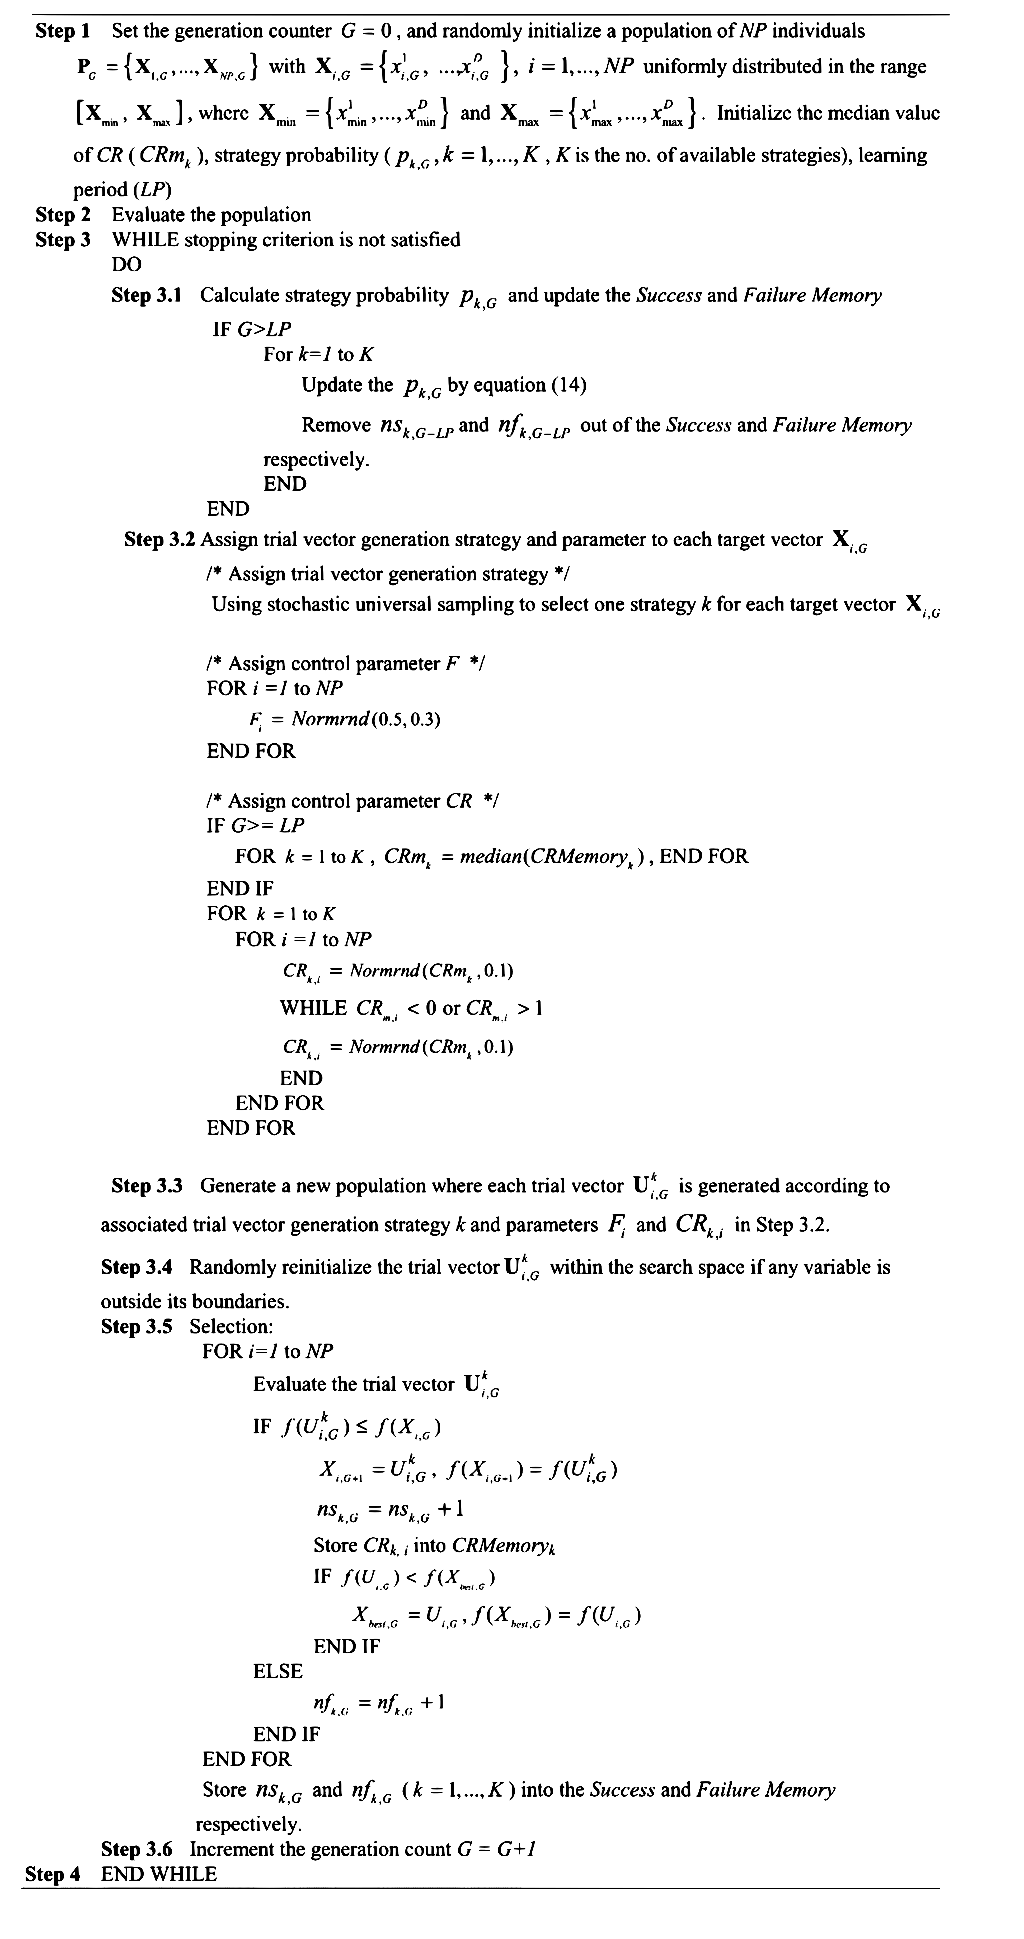
\includegraphics[height=1\textheight]{alg-v.png}
   \captionof{figure}{الگوریتم \lr{SaDE}}
\label{fig:sade} 
\end{minipage}
}
\end{figure}

\newpage
\section{آزمایش‌های عددی و ارزیابی}

\subsection{توابع آزمون}

برای ارزیابی الگوریتم‌های بهینه‌سازی عددی، توابع آزمونی\LTRfootnote{ Test functions} وجود دارد که برخی از آن‌ها در زمینه‌ی تکامل تفاضلی استفاده شده‌اند. پژوهشگران مقاله‌ی مورد نظر، به این نکته اشاره نموده‌اند که این توابع دو مشکل عمده دارند. مشکل اول این است که بهینه‌ی سراسری تابع در مرکز قرار دارد. مشکل دوم، وجود بهینه‌ی محلی روی محورهای مختصات، یا به بیان دیگر، عدم وجود ارتباط بین متغیرها و ابعاد است. به این معنی که قرار گرفتن در آن بُعد، راهی برای خروج در طول بهینه‌سازی عددی و منتقل شدن به ابعاد دیگر نخواهد داشت. برای حل این دو مشکل، توابع معمول بر اساس وجود مشکل جابه‌جا یا دوران‌داده شده‌اند. 

برای توابعی که مشکل اول را دارند، بهینه‌ی سراسری به مکانی تصادفی جابه‌جا می‌شود، به‌گونه‌ای که در ابعاد مختلف مقادیر مختلف داشته باشد. برای مثال، 
$F(x) = f(x - o_{new} + o_{old})$
در نظر گرفته‌‌می‌شود که در آن 
$F(x)$
تابع جدید، 
$f(x)$
تابع اصلی، 
$o_{old}$
بهینه‌ی سراسری اصلی و 
$o_{new}$
بهینه‌ی سراسری جدید است که مقادیرش در ابعاد مختلف، متفاوت است و در مرکز بازه‌ی جست‌وجو نیست. برای توابعی که مشکل دوم را دارند، چرخش به صورت 
$F(x) = f(Mx)$
اعمال شده‌است که در آن 
$M$
یک ماتریس دوران قطری است که در عین حفظ خواص تابع آزمون اصلی، از قرار گرفتن بهینه‌ی محلی روی محورهای مختصات جلوگیری می‌کند. در پژوهش انجام‌شده، توابع 
$f_1$
تا 
$f_5$
، 
$f_7$، 
$f_9$، 
$f_{11} $
و 
$f_{12} $
جابه‌جا شده‌اند و توابع 
$f_6$، 
$f_8 $
و 
$f_{10}$
دوران‌داده شده‌اند. 
توابع 
$f_1 $
تا 
$f_4 $
تک‌قله‌ای و توابع 
$f_5 $
تا 
$f_{14}$
چندقله‌ای هستند. 
توابع آزمون در ادامه آورده شده‌اند. 
\begin{enumerate}
		\item
		تابع کره‌ی جابجا شده
		\begin{align*}
			f_1(x) &=\sum_{i=1}^D{z_i^2}\\
			z &= x - o \\
			o &= [o_1, o_2, ...,o_D] : \text{ بهینه‌ی سراسری جابجا شده}
		\end{align*}

		
		\item
		\lr{Schwefel} جابجا شده‌ی مساله‌ی ۱.۲
		\begin{align*}
			f_2(x) &=\sum_{i=1}^{D-1}\left({\sum_{j=1}^i {z_j}}\right)^2\\
			z &= x - o \\
			o &= [o_1, o_2, ...,o_D] : \text{ بهینه‌ی سراسری جابجا شده}
		\end{align*}
		
		\item
		 تابع \lr{Rosenbrock}
		\begin{align*}
			f_3(x) &=\sum_{i=1}^{D-1}\left(100(x_i^2-x_{i+1})^2 + (x_i - 1)^2 \right)
		\end{align*}
		
		\item
		تابع
		\lr{Schwefel}
		 مسئله‌ی ۱.۲ به همراه نویز در تابع شایستگی
		\begin{align*}
			f_4(x) &=\left( \sum_{i=1}^D\left(\sum_{j=1}^i {z_j}\right)^2\right) (1+0.4)\left|N(0,1)\right|)\\
			z &= x - o \\
			o &= [o_1, o_2, ...,o_D] : \text{ بهینه‌ی سراسری جابجا شده}
		\end{align*}
		
		\item
		 تابع
		\lr{Ackly}
		جابجا شده
		\begin{align*}
			f_5(x) &= -20 \exp\left({-0.2\sqrt{\frac{1}{D}\sum_{i=1}^D z_i^2}}\right) -\exp\left({\frac{1}{D} \sum_{i=1}^D cos(2\pi z_i)} \right) + 20 + e,\\
					 z &= x - o \\
					o &= [o_1, o_2, ...,o_D] : \text{ بهینه‌ی سراسری جابجا شده}
		\end{align*}	
		
		
		
		\item
		  تابع دوران‌یافته و جابجا‌شده‌ی 
		\lr{Ackly} 
		\begin{align*}
			f_6(x) &=
			-20 \exp\left({-0.2\sqrt{\frac{1}{D}\sum_{i=1}^D z_i^2}}\right) -\exp\left({\frac{1}{D} \sum_{i=1}^D cos(2\pi z_i)} \right) + 20 + e,\\
			z &= M(x - o), \text{\lr{cond(M)= 1}} \\
			o &= [o_1, o_2, ...,o_D] : \text{ بهینه‌ی سراسری جابجا شده}
		\end{align*}		
		
		\item
		  تابع جابجا‌شده‌ی
		\lr{Griewank}
		\begin{align*}
			f_7(x) &=\sum_{i=1}^D{\frac{z_i^2}{4000}}\\
			z &= x - o \\
			o &= [o_1, o_2, ...,o_D] : \text{ بهینه‌ی سراسری جابجا شده}
		\end{align*}		
		
		
		\item
		  تابع دوران‌یافته و جابجا‌شده‌ی
		\lr{Griewank}
		\begin{align*}
			f_8(x) &=\sum_{i=1}^D{\frac{z_i^2}{4000}}\\
			z &= M(x - o), \text{\lr{cond(M) = 3}} \\
			o &= [o_1, o_2, ...,o_D] : \text{ بهینه‌ی سراسری جابجا شده}
		\end{align*}
		
		
		\item
		  تابع جابجا‌شده‌ی
		\lr{Rastrigin}
		\begin{align*}
			f_9(x) &=\sum_{i=1}^D{(z_i^2-10cos(2\pi z_i) + 10)}\\
			z &= M(x - o), \text{\lr{cond(M) = 2}} \\
			o &= [o_1, o_2, ...,o_D] : \text{ بهینه‌ی سراسری جابجا شده}
		\end{align*}
		
		\item
		  تابع دوران‌یافته و جابجا‌شده‌ی 
		\lr{Rastrigin}
		\begin{align*}
			f_{10}(x) &=\sum_{i=1}^D{(z_i^2-10cos(2\pi z_i) + 10)}\\
			z &= M(x - o), \text{\lr{cond(M) = 2}} \\
			o &= [o_1, o_2, ...,o_D] : \text{ بهینه‌ی سراسری جابجا شده}
		\end{align*}
		
		
		\item
		  تابع  جابجا‌شده‌ی ناپیوسته
		\lr{Rastrigin}
		\begin{align*}
			f_{11}(x) &=\sum_{i=1}^D{(y_i^2-10cos(2\pi z_i) + 10)}\\
			y_i &=
			\begin{cases}
				z_i, &|z_i| < 1/2 \\
				round(2 z_i)/2, &|z_i| >= 1/2 \\
			\end{cases} 
			\\
			& \hspace{5cm} \text{\lr{for i = 1,2, ...,D}}			
			\\
			z &= M(x - o), \text{\lr{cond(M) = 2}} \\
			o &= [o_1, o_2, ...,o_D] : \text{ بهینه‌ی سراسری جابجا شده}
		\end{align*}
		
		\item
		  تابع
		\lr{Schwefel}
		\begin{align*}
		f_{12}(x) = 418.9829 \times D - \sum_{i=1}^D x_i sin\left(|x_i|^{1/2} \right)
		\end{align*}
		
		\item 
		$f_{13}$
		تابع مرکب شماره‌ی ۱ است که در \cite{32-cf} معرفی شده‌است. در آن مقاله، شش تابع پایه‌ معرفی شده‌است و روشی برای ترکیب آن‌ها ارایه شده‌است. تابع مرکب شماره‌ی ۱، از ترکیب ده تابع کره به‌دست می‌آید که در شکل \ref{fig:cf1} شمای کلی آن‌ را می‌بینید.
		\begin{figure}[!hbtp]
		\centering
		\caption{تابع مرکب شماره‌ی ۱ \cite{32-cf}}
		\label{fig:cf1}
		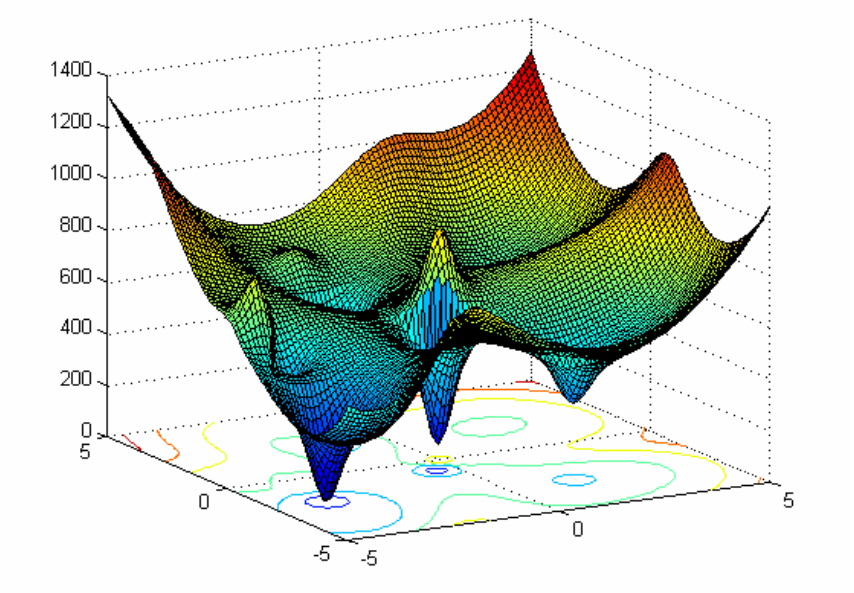
\includegraphics[height=7cm]{cf1.png}
		\end{figure}
   
		\item 
		$f_{14}$
		تابع مرکب شماره‌ی ۶ است که در \cite{32-cf} معرفی شده‌است. این تابع با ترکیب ده تابع آزمون گوناگون به‌دست آمده‌است. توابع
		\lr{Rastrigin}،
		\lr{Rastrigin}،
		\lr{Weierstrass}،
		\lr{Griewank} به صورت دوران‌داده شده
		و تابع کره، ترکیب شده‌اند. هر تابع دو مرتبه استفاده شده‌است. شمای کلی این تابع را در شکل \ref{fig:cf6} می‌بینید.

		\begin{figure}[!hbtp]
		\centering
		\caption{تابع مرکب شماره‌ی ۶ \cite{32-cf}}
		\label{fig:cf6}
		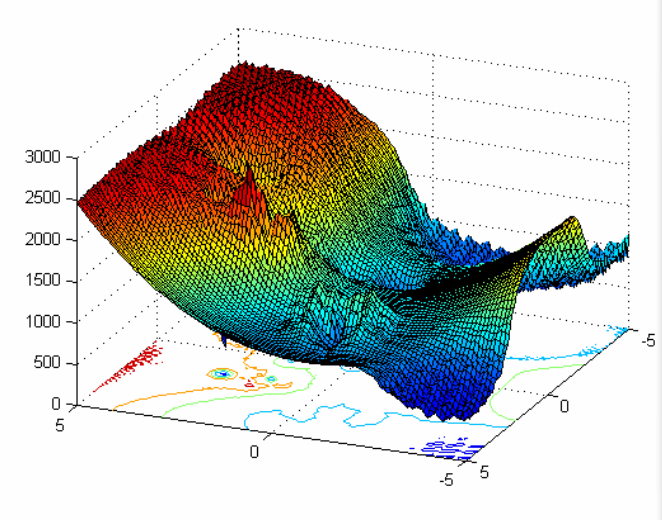
\includegraphics[height=7cm]{cf6.png}
		\end{figure} 
		
		\item
		  تابع
		\lr{Schwefel}
		 مساله‌ی ۲.۲۲
		\begin{align*}
		f_{15}(x) = \sum_{i=1}^D |x_i| + \prod_{i=1}^D |x_i|
		\end{align*}
		
		\item
		  تابع
		\lr{Schwefel}
		 مساله‌ی ۲.۲۱
		\begin{align*}
		f_{16}(x) = \max_{i}\{ |x_i|, 1 \le i \le D\}
		\end{align*}
		
		
		\item
		  تابع ۱ جریمه شده‌ و عمومی شده
		
		\noindent\makebox[\textwidth][c]{%
		\begin{minipage}[h][][b]{1.3\textwidth}
		\begin{align*}
		f_{17}(x) &= 
		\frac{\pi}{D} \left\{ 10 sin^2(\pi y_1) + \sum_{i=1}^{D-1}(y_i - 1)^2  \times [1 + 10 sin^2(\pi y_{i+1})  + (y_D -1)] \right\} \\
		\\ 
		& \quad + \sum_{i=1}^D u(x_i, 10, 100, 4)\\
		y_i &= 1 + \frac{1}{4}(x_i + 1)\\
				u(x_i,10, 100, 4) & = 
			\begin{cases}
				k(x_i = a)^m, & x_i >2 \\
				0, & -a \le x_i \le a \\
				k(-x_i-a)^m, & x_i < a
			\end{cases}
		\end{align*}
		\end{minipage}
		}
		
		\item
		   تابع ۲ جریمه شده‌ و عمومی شده
		
		\noindent\makebox[\textwidth][c]{%
		\begin{minipage}[h][][b]{1.3\textwidth}
		\begin{align*}
		f_{18}(x) = 0.1 \left\{ sin^2(3\pi x_1) + \sum_{i=1}^{D-1} (x_i - 1)^2 [1 + sin^2(3\pi x_{i+1})] \right. \\
		 \left. + (x_D-1)[1 + sin^2(2\pi x_D) {\vphantom{\sum_{i=1}^{D-1} }} \right\} + \sum_{i=1}^D u(x_i, 5, 100, 4)
		\end{align*}
		\end{minipage}
		}

		
		\item
		  تابع
		\lr{Kowalik}
		\begin{align*}
		f_{19}(x) = \sum_{i=1}^{11} \left[ a_i - \frac{x_1(b_i^2 + b_ix_2)}{b_i^2 + b_i x_3 + x_4} \right]^2
		\end{align*}
		
		
		\item
		  تابع
		\lr{Six-hump camel-back}
		\begin{align*}
		f_{20} (x) = 4x_1^2 - 2.1x_1^4 + \frac{1}{3}x_1^6 + x_1x_2 - 4x_2^2 + 4x_2^4
		\end{align*}
		
		
		\item
		  تابع
		\lr{Brainin}
		\begin{align*}
		f_{21} (x)  = \left( x_2 - \frac{5.1}{4\pi^2}x_1^2 + \frac{5}{\pi}x_1 - 6 \right)^2 + 10 \left( 1- \frac{1}{8\pi}\right)cos x_1 + 10
		\end{align*}
		
		
		\item
		  تابع اول
	    \lr{Hartman} 
		\begin{align*}
		f_{22} (x) = -\sum_{i=1}^{4} c_i \exp\left[ -\sum_{j=1}^3 a_{ij}(x_j - p_{ij})^2\right]
		\end{align*}
		
		
		\item
		  تابع دوم
		\lr{Hartman}
		\begin{align*}
		f_{23} (x)  = -\sum_{i=1}^{4} c_i \exp\left[ -\sum_{j=1}^6 a_{ij}(x_j - p_{ij})^2\right]
		\end{align*}
		
		
		\item
		  خانواده
		\lr{Shekel}
		\begin{align*}
		f(x)  = - \sum_{i=1}^m{[(x-a_i)^T(x-a_i) + c_i]^{-1}},
		\end{align*}
		با 
		$m=5,7 , 10$
		برای توابع
		$f_{24}(x)$،
		$f_{25}(x)$
		و 
		$f_{26}(x)$ . 

\end{enumerate}

\subsection{‌الگوریتم‌های مقایسه‌شده}

مقاله‌ی مورد نظر، نتایج اجرای توابع آزمون بر روی روش ارایه‌شده را با ۸ الگوریتم دیگر مقایسه نموده‌است که این مقایسه، برای توابع 
$f_1$
تا 
$f_{14}$
هم در حالت ۱۰بعدی و هم در حالت ۳۰بعدی انجام شده‌است. تعداد بیشینه‌ی فراخوانی ارزیابی‌ برای یک تابع \lr{(FEs)}\LTRfootnote{ Function evaluations} در حالت ۱۰بعدی برابر با ۱۰۰۰۰۰ و در حالت ۳۰بعدی برابر با ۳۰۰۰۰۰ قرارداده‌ شده‌است. برای توابع باقی‌مانده
$f_{15}$
تا 
$f_{26}$
، ابعاد در جدول \ref{tab:dims} آورده شده‌است. همچنین بیشینه‌ی فراخوانی ارزیابی برای این توابع برابر با ۵۰۰۰۰۰ قرارداده شده‌است. تمامی آزمایش‌ها ۳۰ بار به طور مستقل انجام شده‌است. الگوریتم‌های مقایسه‌شده عبارت‌اند از: 
\begin{enumerate}
\item
\lr{DE/rand/1/bin} : $F = 0.9, CR = 0.1$

\item
\lr{DE/rand/1/bin} : $F = 0.9, CR = 0.9$

\item
\lr{DE/rand/1/bin} : $F = 0.5, CR = 0.3$

\item
\lr{DE/rand-to-best/1/bin} : $F = 0.5, CR = 0.3$

\item
\lr{DE/rand-to-best/2/bin} : $F = 0.5, CR = 0.3$

\item
تکامل تفاضلی تطبیقی یا
\lr{ADE} \cite{demon4}

\item
روش 
\lr{SDE} \cite{27}

\item
روش
\lr{jDE} \cite{28}
\end{enumerate}


در تمامی حالات آزمایش‌ها، تعداد جمعیت ۵۰ و دوره‌ی یادگیری
$\mathit{LP}$
نیز برابر با ۵۰ قرارداده شده‌است. 

با توجه به کارهای انجام‌شده در تکامل تفاضلی دیدیم که روش‌های ۱ تا ۳ با مقادیر پارامترهای به‌کاربرده شده، از پرکاربردترین روش‌ها در تکامل تفاضلی هستند و روش ۴ و ۵، از استراتژی‌های بهبودیافته‌ی پرکاربرد بودند. پژوهشگران این مقاله، روش‌های ۶ تا ۸ را نیز به دلیل تطبیقی بودنشان انتخاب نموده‌اند و تا همین‌جا می‌توان به قوی بودن آزمایش‌های انجام‌شده پی‌برد که به جرات نقطه‌ی قوت اصلی مقاله‌ی انتخابی است. 

\renewcommand{\arraystretch}{1.5}
\noindent
\begin{table}[!htbp]
\footnotesize
\caption{\small{بهینه‌ی سراسری، بازه‌های جست‌و‌جو، و بازه‌های مقداردهی اولیه‌ی توابع آزمون}}

%\textsuperscript{*}}
\centering
\begin{adjustbox}{center}

%\begin{tabular}{ | c | >{\centering}m{0.45\textwidth} | m{0.6\textwidth}| }
\begin{tabular}{ c c c c c c}

\hline
\hline

$f$
& 
بُعد
&
بهینه‌ی سراسری$x^*$
&
$f(x^*)$
&
بازه‌ی جست‌وجو
&
بازه‌ی مقداردهی اولیه
\tabularnewline
\hline
\rowcolor{Gray}
$f_1$
&

&
$\mathit{o}$
&
$0$
&
$[-100, 100]^D$
&
$[-100, 100]^D$
\tabularnewline
\rowcolor{LGray}
$f_2$
&

&
$\mathit{o}$
&
$0$
&
$[-100, 100]^D$
&
$[-100, 100]^D$
\tabularnewline
\rowcolor{Gray}
$f_3$
&

&
$(1,1,\cdots,1)$
&
$0$
&
$[-100, 100]^D$
&
$[-100, 100]^D$
\tabularnewline
\rowcolor{LGray}
$f_4$
&

&
$\mathit{o}$
&
$0$
&
$[-32, 32]^D$
&
$[-32, 32]^D$
\tabularnewline
\rowcolor{Gray}
$f_5$
&

&
$\mathit{o}$
&
$0$
&
$[-32, 32]^D$
&
$[-32, 32]^D$
\tabularnewline
\rowcolor{LGray}
$f_6$
&

&
$\mathit{o}$
&
$0$
&
$\mathfrak{R}$
&
$[0, 600]^D$
\tabularnewline
\rowcolor{Gray}
$f_7$
&
10,30
&
$\mathit{o}$
&
$0$
&
$\mathfrak{R}$
&
$[0, 600]^D$
\tabularnewline

\rowcolor{LGray}
$f_8$
&

&
$\mathit{o}$
&
$0$
&
$[-5,5]^D$
&
$[-5,5]^D$
\tabularnewline


\rowcolor{Gray}
$f_9$
&

&
$\mathit{o}$
&
$0$
&
$[-5,5]^D$
&
$[-5,5]^D$
\tabularnewline

\rowcolor{LGray}
$f_{10}$
&

&
$\mathit{o}$
&
$0$
&
$[-5,5]^D$
&
$[-5,5]^D$
\tabularnewline

\rowcolor{Gray}
$f_{11}$
&

&
$(420.96 , \cdots , 420.96)$
&
$0$
&
$[-500,500]^D$
&
$[-500,500]^D$
\tabularnewline


\rowcolor{LGray}
$f_{12}$
&

&
$(420.96 , \cdots , 420.96)$
&
$0$
&
$[-500,500]^D$
&
$[-500,500]^D$
\tabularnewline

\rowcolor{Gray}
$f_{13}$
&

&
$\mathit{o}_1$
&
$0$
&
$[-5,5]^D$
&
$[-5,5]^D$
\tabularnewline

\rowcolor{LGray}
$f_{14}$
&

&
$\mathit{o}_1$
&
$0$
&
$[-5,5]^D$
&
$[-5,5]^D$
\tabularnewline
\hline 

\rowcolor{Gray}
$f_{15}$
&
30
&
$(0, \cdots , 0)$
&
$0$
&
$[-10,10]^D$
&
\tabularnewline


\rowcolor{LGray}
$f_{16}$
&
30
&
$(0, \cdots , 0)$
&
$0$
&
$[-100,100]^D$
&
\tabularnewline

\rowcolor{Gray}
$f_{17}$
&
30
&
$(1, \cdots , 1)$
&
$0$
&
$[-50,50]^D$
&
\tabularnewline

\rowcolor{LGray}
$f_{18}$
&
30
&
$(1, \cdots , 1)$
&
$0$
&
$[-50,50]^D$
&
\tabularnewline

\rowcolor{Gray}
$f_{19}$
&
4
&
{\footnotesize$(0.1928, 0.1908 , 0.1231 , 0.1358)$}
&
$0.0003075$
&
$[-5,5]^D$
&
\tabularnewline

\rowcolor{LGray}
$f_{20}$
&
2
&
{\footnotesize$(0.8983,-0.7126),(-0.08983,0.7126)$}
&
$-1.0316285$
&
$[-5,5]^D$
&
برابر با بازه‌ی
\tabularnewline

\rowcolor{Gray}
$f_{21}$
&
2
&
{\scriptsize$(-3.142,12.275),(3.142,2.275),(9.425,2.425)$}
&
$0.398$
&
$[-5,10] \times [0,15]$
&
جست‌و‌جو
\tabularnewline

\rowcolor{LGray}
$f_{22}$
&
4
&
$(0.114, 0.556 , 0.825)$
&
$-3.86$
&
$[0,1]^D$
&
\tabularnewline

\rowcolor{Gray}
$f_{23}$
&
6
&
{\scriptsize{$(0.201, 0.150 , 0.477, 0.275, 0.311, 0.657)$}}
&
$-3.32$
&
$[0,1]^D$
&
\tabularnewline

\rowcolor{LGray}
$f_{24}$
&
4
&
$[4,4,4,4]$
&
$-10.2$
&
$[0,10]^D$
&
\tabularnewline

\rowcolor{Gray}
$f_{25}$
&
4
&
$[4,4,4,4]$
&
$-10.4$
&
$[0,10]^D$
&
\tabularnewline


\rowcolor{LGray}
$f_{26}$
&
4
&
$[4,4,4,4]$
&
$-10.5$
&
$[0,10]^D$
&
\tabularnewline

\hline
\end{tabular}
\label{tab:dims}
\end{adjustbox}
\begin{flushright}
\footnotesize{
${\mathit{o}\hphantom{_1}}$
بردارِ جابه‌جاشده‌ است.

$\mathit{o}_1$
بردارِ جابه‌جاشده برای اولین تابعِ بایه در تابع مرکب است.
}

\end{flushright}
\end{table}
\newpage 
\subsection{نتایج آزمایش و تحلیل‌ها}

نتایج اجرای این ۹ الگوریتم و میانگین و انحراف استاندارد آن‌ها در شکل‌ \ref{fig:r1} به طور مستقیم از مقاله‌ی مورد بررسی آورده شده‌است. جداول برای ده بعد و سی بعد هستند و شامل نتایج برای 
$f_1$
تا 
$f_{14}$
هستند و بهترین نتایج پررنگ شده‌اند. موفقیت الگوریتم‌ها این‌گونه تعریف شده‌است که بتوانند به مقدار بهینه‌ی از پیش تعریف‌شده مانند 
$f(x^*)+1 e -5$
برای تمامی توابع آزمون برسند، و این کار را با تعداد ارزیابی‌هایی کمتر از تعداد ارزیابی بیشینه انجام دهند. نرخ موفقیت نیز با تقسیم تعداد اجراهای موفقیت‌آمیز بر تعداد کل اجراها به‌دست آمده‌است. 

\begin{figure}
\noindent\makebox[\textwidth][c]{
\vspace{-3cm}
\begin{minipage}[h][][b]{1.3\textwidth}
   \vspace{-2ex}
   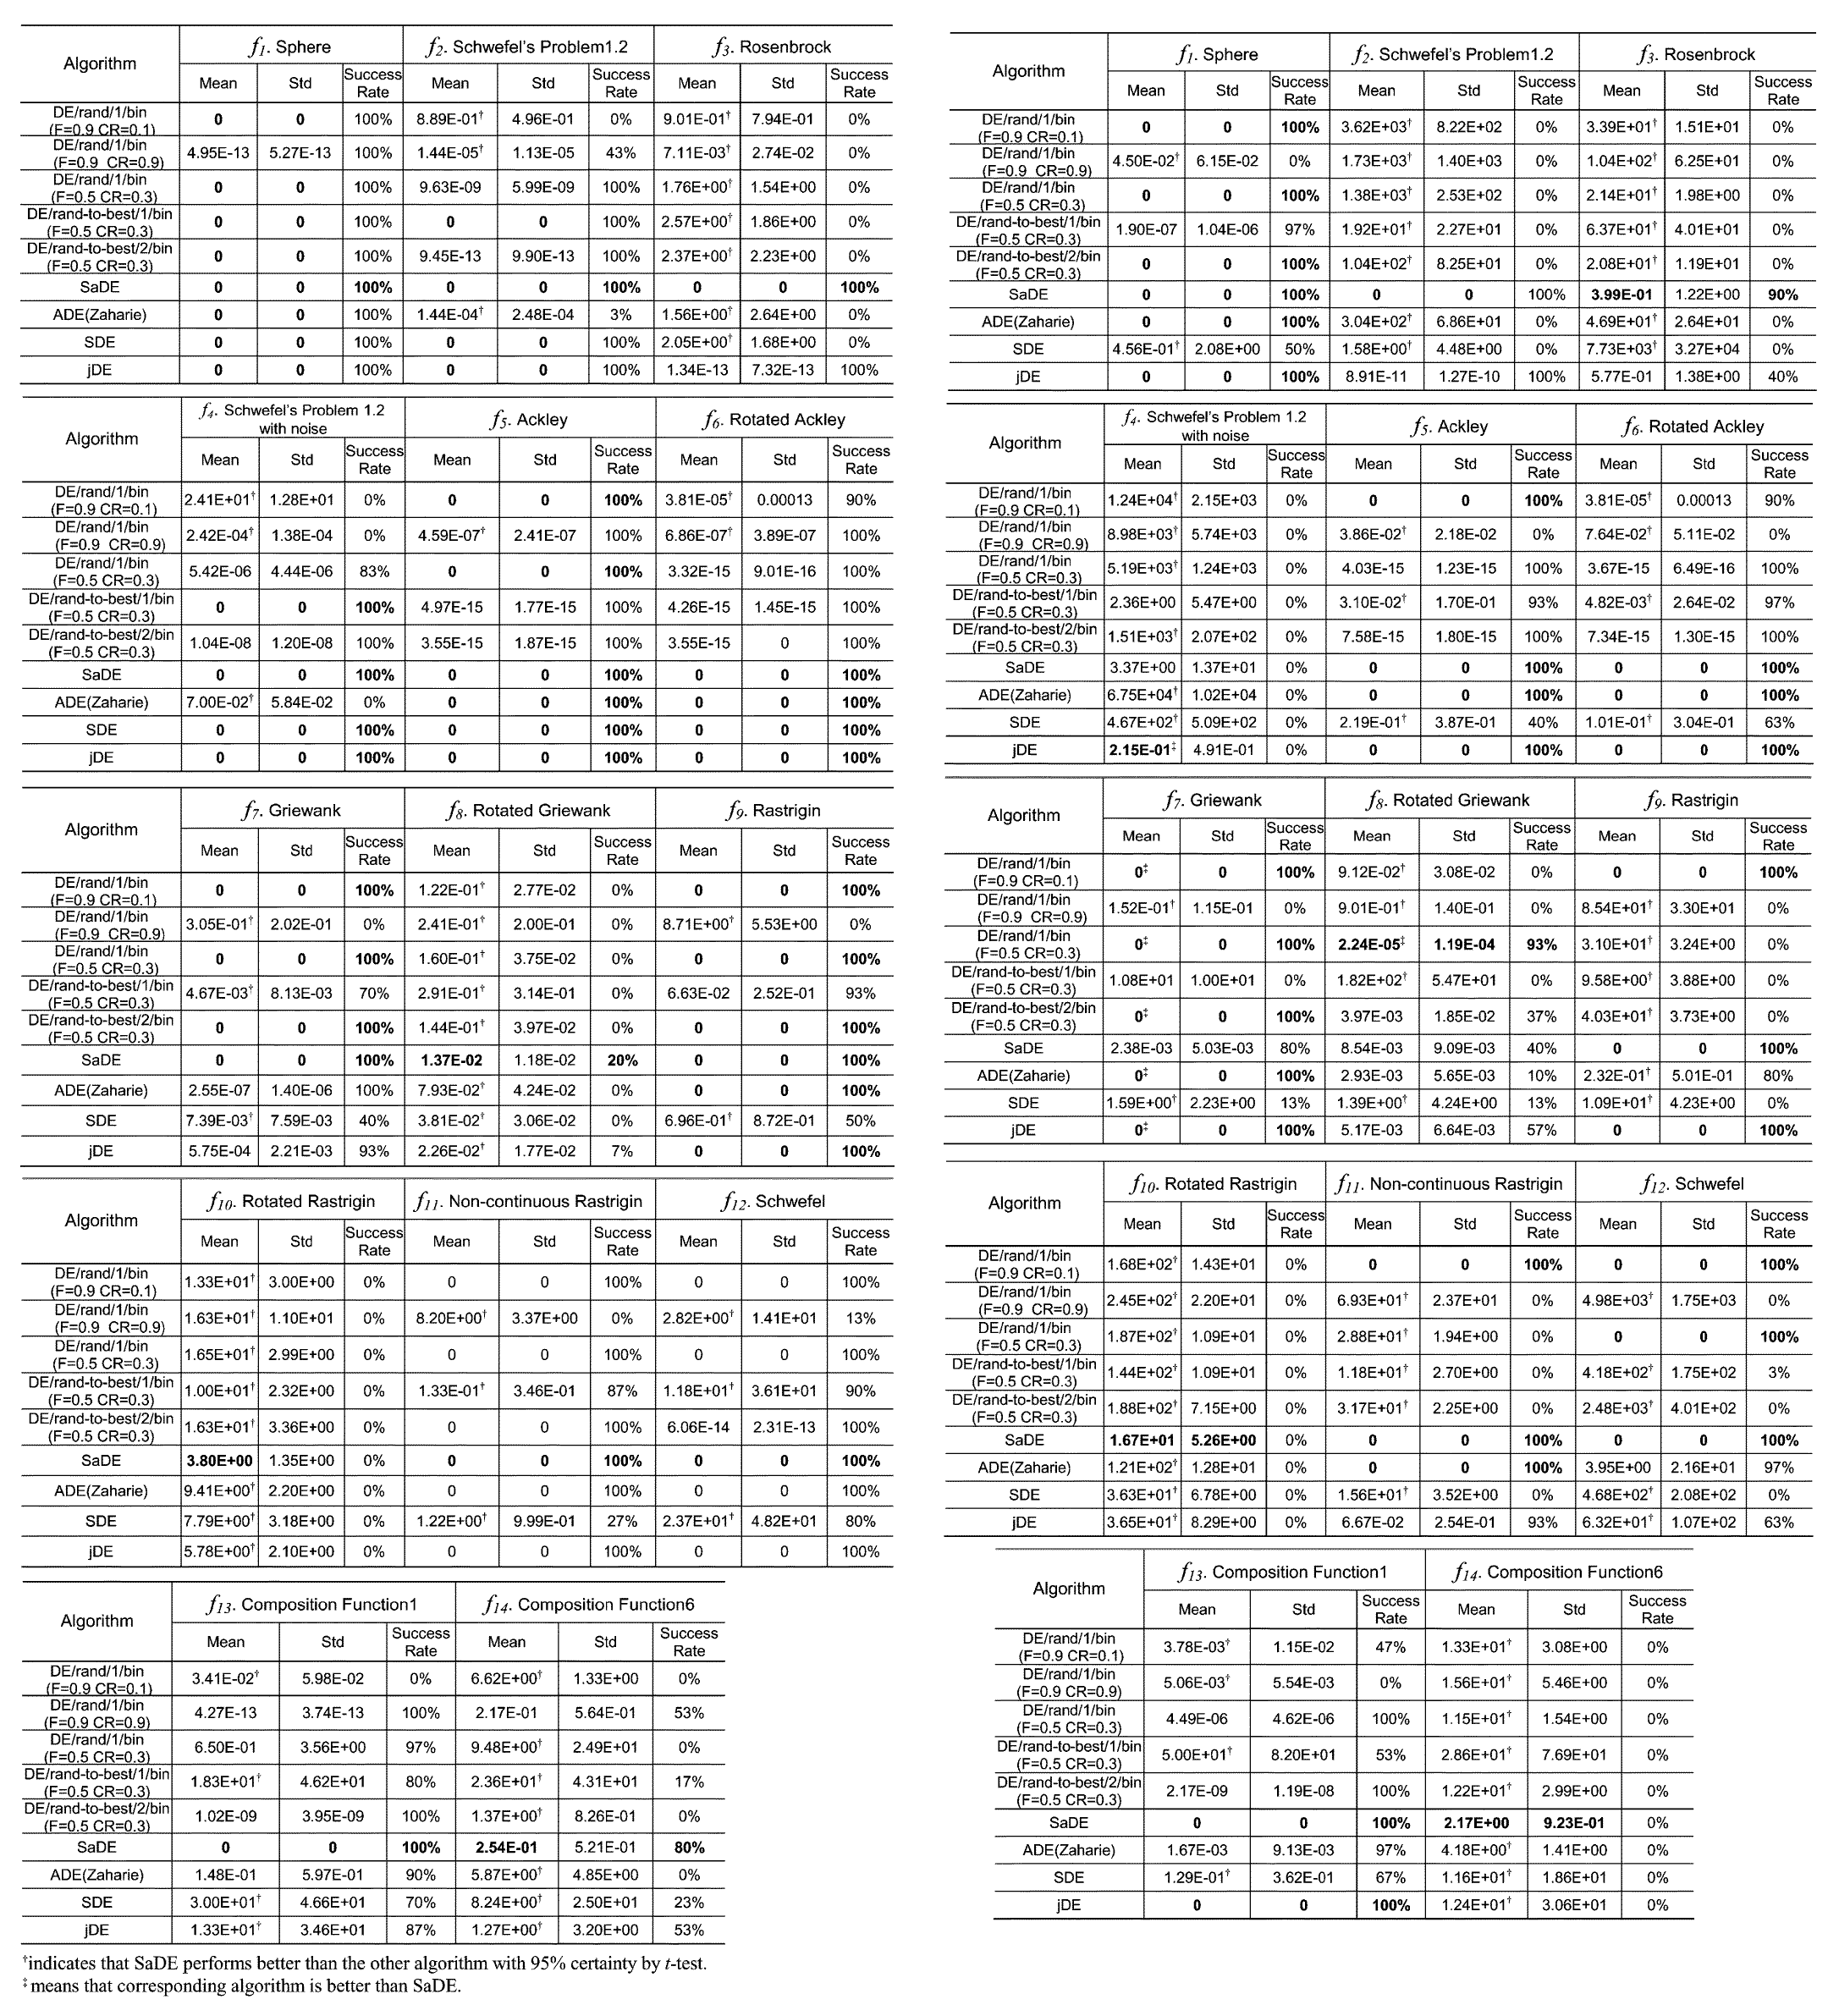
\includegraphics{r1.png}
   \captionof{figure}{نتایج برای ده بعد (سمت چپ) و سی بعد (سمت راست)}
\label{fig:r1} 
\end{minipage}
}
\end{figure}

تصاویر \ref{fig:r2} و \ref{fig:r3} همگرایی را برای بهترین برازش و به ازای میانه‌ی اجراها با 
$D=10$
نشان می‌دهد. پژوهشگران مقاله نتایج برای سی‌ بعد را در این جا حذف نموده‌اند چون نمودار همگرایی آن‌ها شبیه به همین نمودارها برای ده بعد است. به همین دلیل، برای مقایسه‌ی همگرایی آن‌ها از مقدار متوسط تعداد ارزیابی‌ها هنگامی که به موفقیت ۱۰۰٪ می‌رسند استفاده شده‌است.
(حروف لاتین به ترتیب نشان‌دهنده‌ی توابع آزمون از 
$f_1$
تا 
$f_{14}$
هستند.)
\begin{figure}
\noindent\makebox[\textwidth][c]{
\begin{minipage}[h][][b]{\textwidth}
   \vspace{-2ex}
   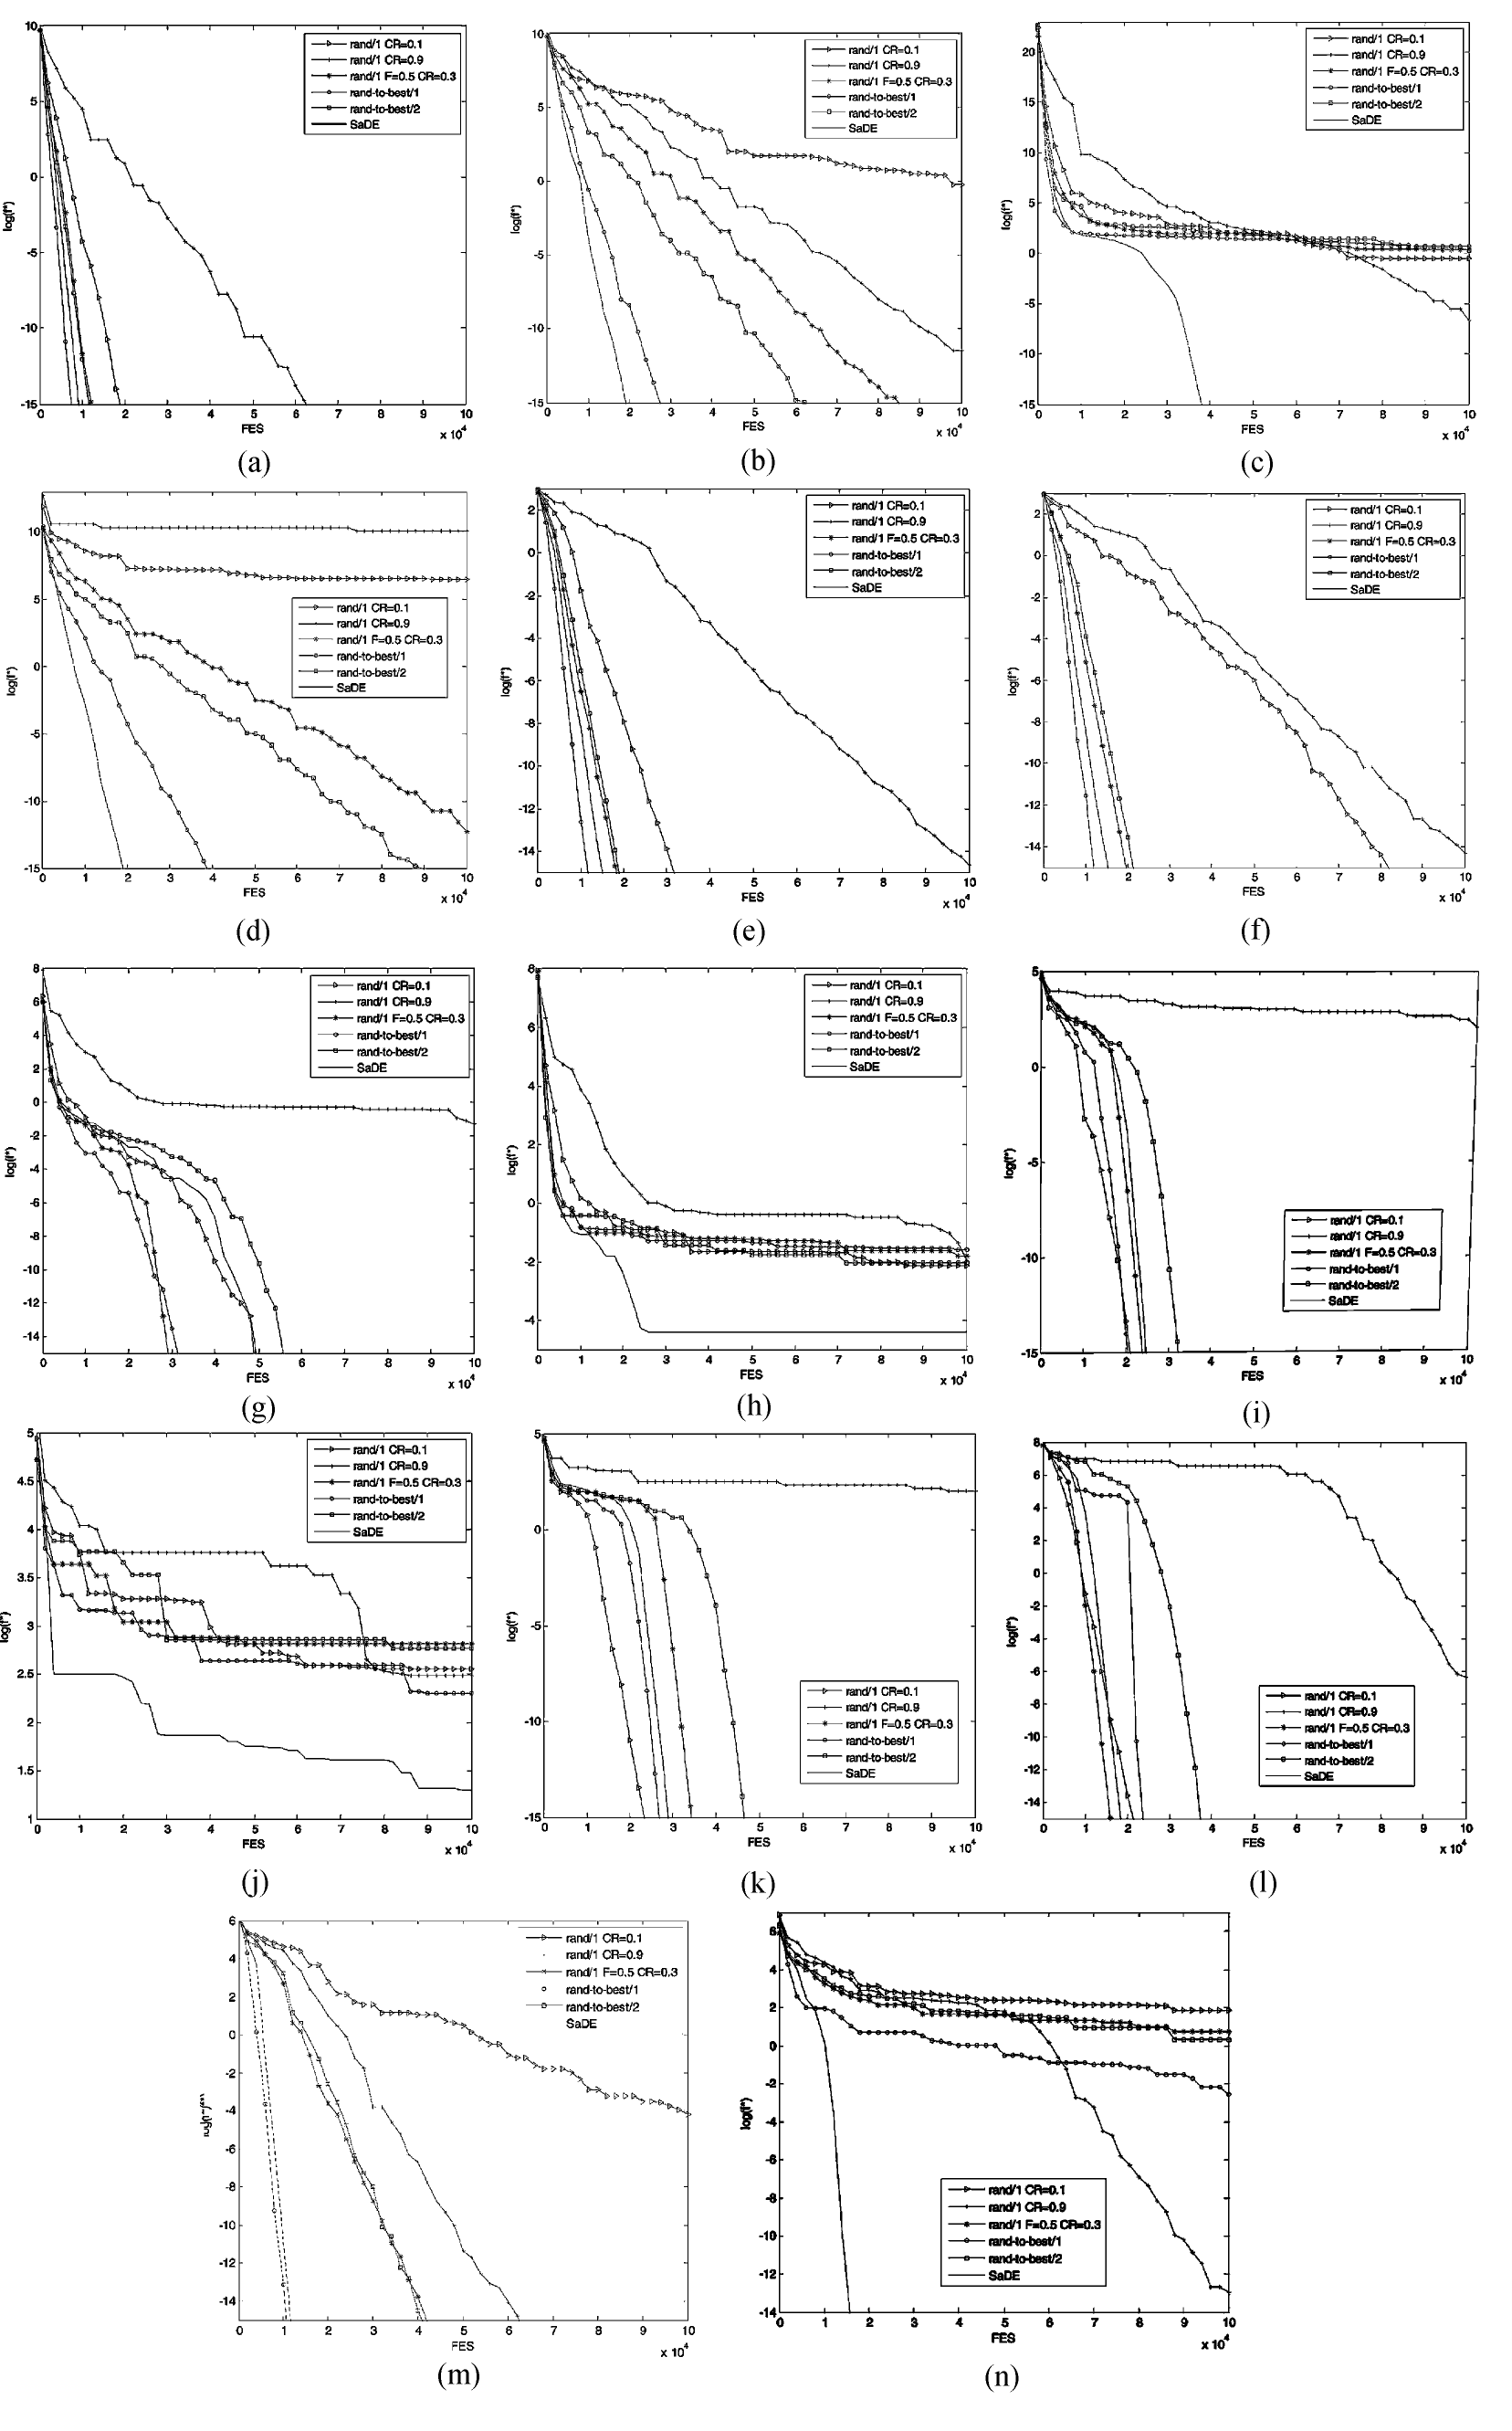
\includegraphics[height=1\textheight]{r2.png}
   \captionof{figure}{نتایج همگرایی الگوریتم‌های معمول برای $f_1$ تا $f_{14}$}
\label{fig:r2} 
\end{minipage}
}
\end{figure}

\begin{figure}
\noindent\makebox[\textwidth][c]{
\begin{minipage}[h][][b]{\textwidth}
   \vspace{-2ex}
   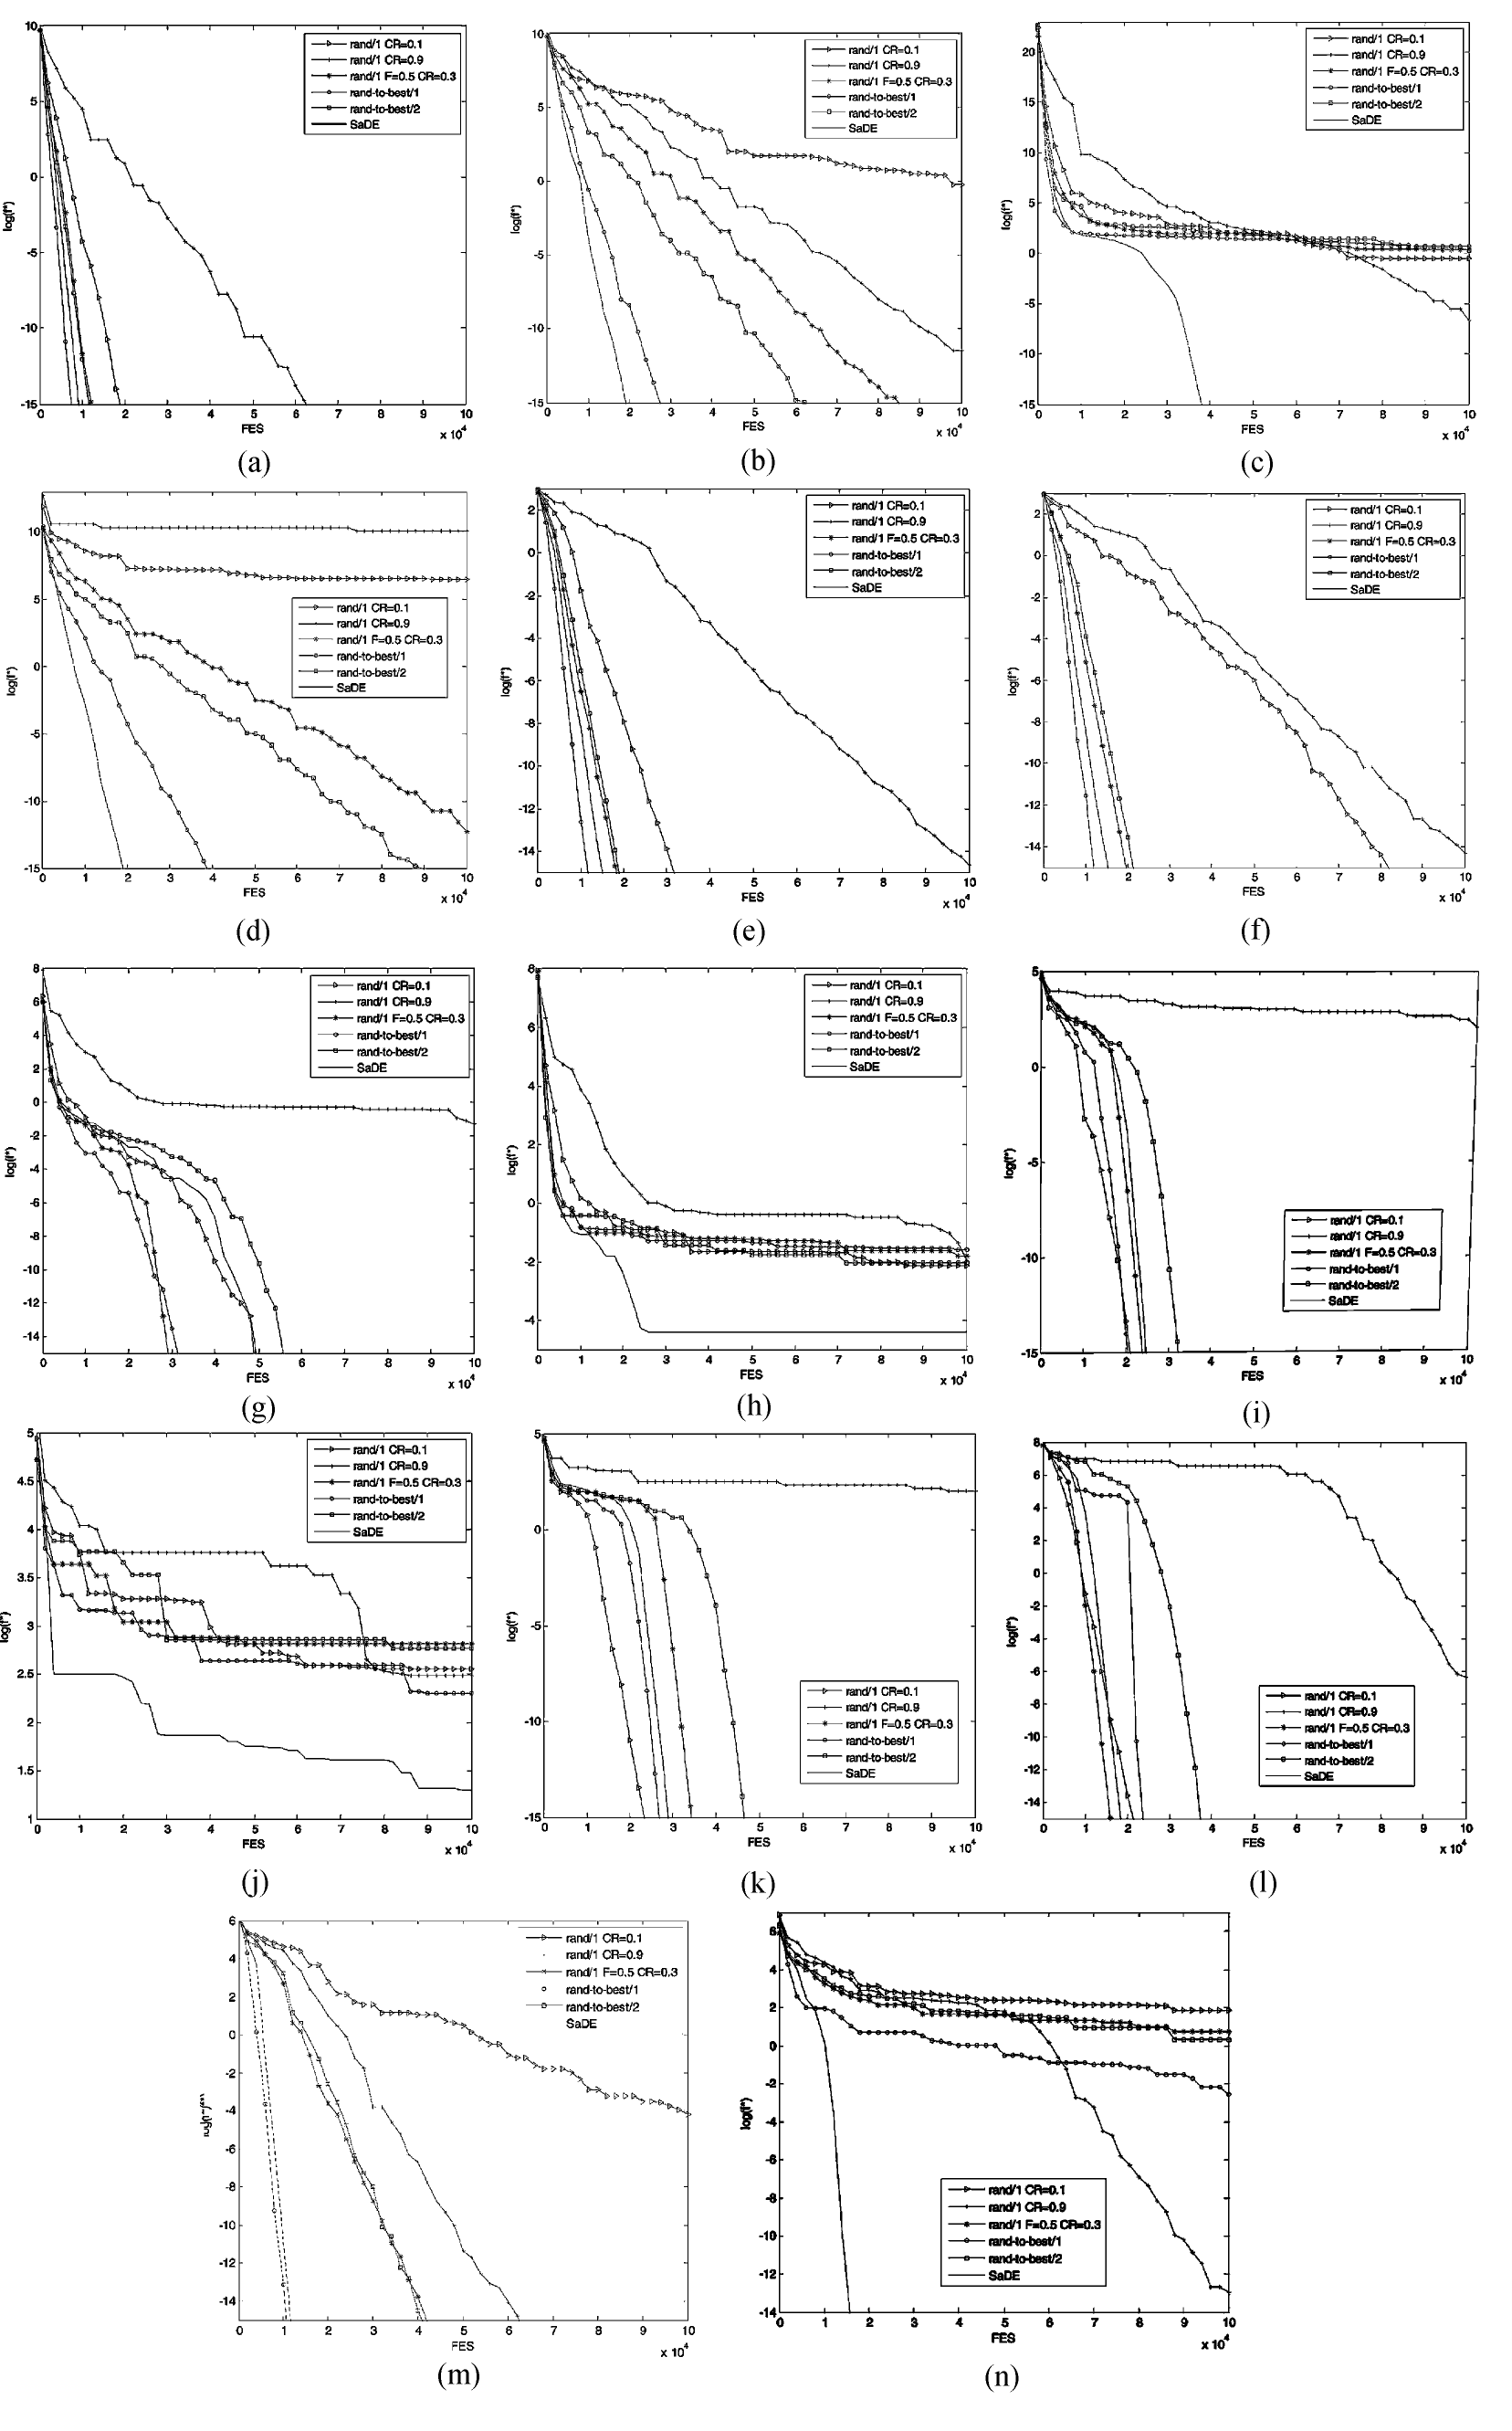
\includegraphics[height=1\textheight]{r2.png}
   \captionof{figure}{نتایج همگرایی الگوریتم‌های تطبیقی برای $f_1$ تا $f_{14}$}
\label{fig:r3} 
\end{minipage}
}
\end{figure}
\subsubsection{مقایسه‌ با روش‌های معمول}
مقایسه‌ها در کل به دو دسته‌ی مقایسه‌ با روش‌های معمول و روش‌های تطبیقی تقسیم شده‌است. مشاهده می‌شود که الگوریتم ارایه‌شده در مجموع میانگین کمتر و نرخ موفقیت بیشتری از راه‌حل‌های معمول تکامل تفاضلی داشته‌است.


\begin{figure}
\noindent\makebox[\textwidth][c]{
\begin{minipage}[h][][b]{\textwidth}
   \vspace{-2ex}
   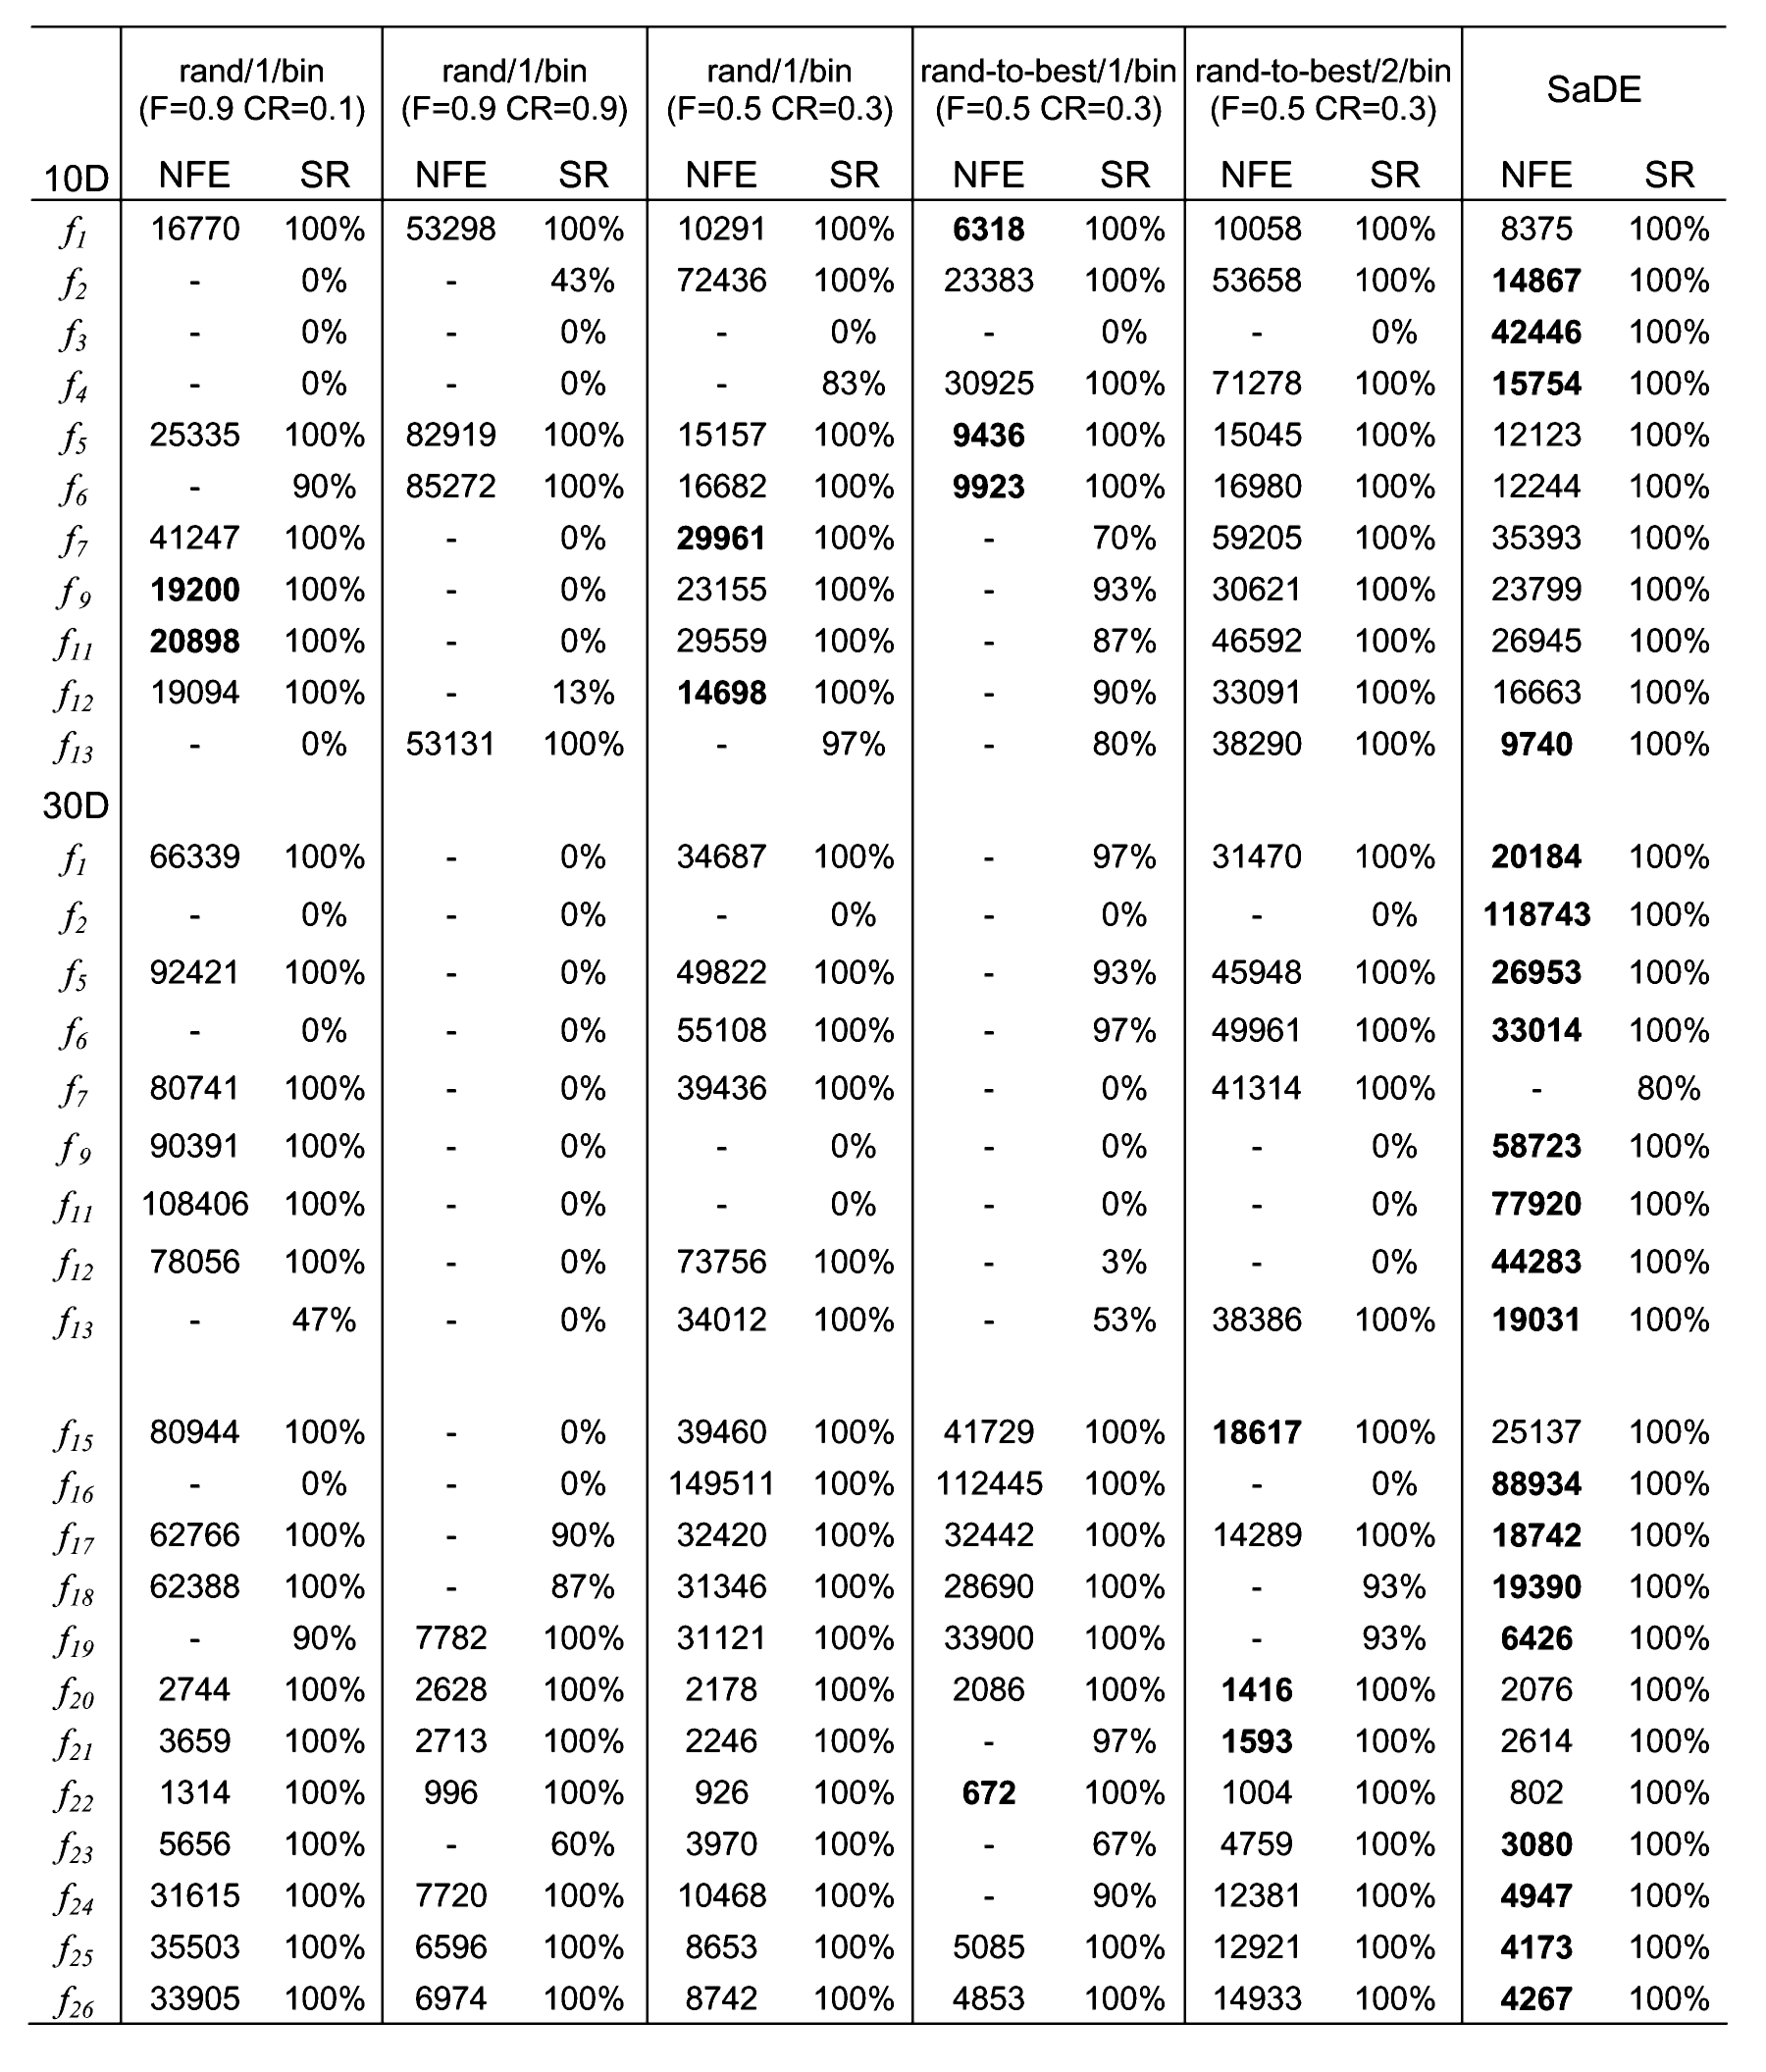
\includegraphics[width=\textwidth]{r4.png}
   \captionof{figure}{مقایسه‌ی سرعت روش پیشنهادی با روش‌های معمول تکامل تفاضلی}
\label{fig:r4} 
\end{minipage}
}
\end{figure}
برای توابع 
$f_{15}$
تا 
$f_{26}$
، از آن‌جا که اغلبشان بهینه‌ی سراسری را در تعداد مناسبی تکرار پیدا می‌کنند، نتایج میانگین و انحراف استاندارد آورده نشده‌است. 

در مورد همگرایی الگوریتم ارایه‌شده، با دقت در شکل \ref{fig:r2} می‌توان دریافت که در توابع آزمون 
$f_2$، 
$f_3$، 
$f_4$، 
$f_8$، 
$f_{10}$ و
$f_{14}$
همیشه سریع‌تر همگرا می‌شود، در حالی که در بقیه‌ی توابع آزمون، همیشه از 
\lr{DE/rand-to-best/1/bin}
و 
\lr{DE/rand/1/bin}
با پارامترهای یادشده، دیرتر همگرا می‌شود.


در مسایل ۳۰ بعدی، 
\lr{DE/rand/1/bin}
در تمام مسایل برای پیدا کردن بهینه‌ی سراسری با مشکل روبه‌رو شده‌است. در حالی که \lr{SaDE} بیشتر توابع آزمون را با نرخ ۱۰۰٪ موفقیت بهینه کرده‌است و تنها برای 
$f_3$ 
به موفقیت ۹۰٪ رسیده‌است که دیگر الگوریتم‌های معمول در آن‌جا کاملا شکست خورده‌اند. جالب آن‌جاست که در حالت ۳۰ بعدی، 
$f_4$،
$f_{10}$، 
و 
$f_{14}$
به قدری سخت شده‌اند که هیچ‌کدام از روش‌های موجود قادر به پیدا کردن بهینه بدون تجاوز از تعداد مجاز ارزیابی نبوده‌اند!

برای مقایسه‌ی سرعت همگرایی‌ها، شکل \ref{fig:r4} تعداد ارزیابی‌ها و نرخ موفقیت‌های ۱۰۰٪ را مقایسه نموده‌است. مشاهده می‌شود که تنها در 
$f_7$، 
الگوریتم ارایه‌شده از دیگر الگوریتم‌ها کندتر بوده‌است و در باقی آزمون‌ها موفق‌تر عمل‌ کرده‌است. 
\subsubsection{مقایسه‌ با روش‌های تطبیقی}
در مقایسه‌ی 
\lr{SaDE}
با دیگر الگوریتم‌های تطبیقی، که 
\lr{jDE}،
\lr{SDE} و 
\lr{ADE}
هستند، بهترین پاسخ‌ها برای ۱۰ بعد و توابع تک‌قله‌ای 
$f_{1}$، 
تا
$f_{4}$
توسط 
\lr{SaDE}
و
\lr{jDE}
به‌دست آمده‌است که با توجه به سرعت همگرایی شکل \ref{fig:r3}، الگوریتم ارایه‌شده کمی برتری دارد. با توجه به شکل \ref{fig:r1} نیز می‌توان دریافت که در توابع 
$f_7$
و 
$f_{9}$
تا قبل از چرخش، همه‌ی روش‌ها پاسخ‌ موفق بوده‌اند اما پس از چرخش، یعنی توابع 
$f_8$
و 
$f_{10}$
تنها 
\lr{SaDE}
و
\lr{jDE}
پاسخ‌گو بوده‌اند و آن‌هم در مورد $f_{10}$ هیچ‌کدام موفق نبوده‌اند و به نظر می‌رسد این‌که پژوهشگران مقاله‌ی مورد نظر در این‌جا برتری را برای روش خود دانسته‌اند، تنها معیار ممکن برای چنین تحلیلی میانگین نزدیک‌تر به بهینه‌ی سراسری و انحراف استاندارد بوده‌است که توسط روش حاصل شده‌است. 

در شکل \ref{fig:r1} می‌توان دید که روش ارایه‌شده در سی بعد برای 
$f_4$،
$f_{10}$
و 
$f_{14}$
نسبت به دیگر روش‌های تطبیقی اصلا موفق نبوده‌است، هرچند نسبت به دیگر روش‌ها میانگین و انحراف استاندارد بهتری داشته‌است، به جز برای 
$f_{14}$
که تنها 
\lr{jDE}
از روش ارایه‌شده مقادیر بهتری را به‌دست داده‌است. 

\subsubsection{مقایسه‌ی کارایی کلی:}

برای مقایسه‌ی کارایی ۹ الگوریتم مورد بررسی، پژوهشگران مقاله از روش رسم توزیع نمونه‌ای\LTRfootnote{ Empirical distribution} کاراییِ موفقیت نرمال‌شده‌ استفاده کرده‌اند که در \cite{36} معرفی شده‌است. این روش کارایی موفقیت \lr{(SP)} را به صورت زیر تعریف نموده‌است: 

\begin{equation}
SP = mean(\mathit{FEs}) \times {{\#total runs} \over {\#successful runs}}
\end{equation}

همان‌گونه که مشاهده می‌شود، این معیار از حاصل‌ضرب میانه‌ی تعداد ارزیابی‌ها در نرخ موفقیت است. با کمی تامل در این فرمول، می‌توانیم به این نکته پی ببریم که اگر نرخ موفقیت الگوریتمی کم باشد اما میانه‌ی تعداد ارزیابی‌های آن نیز کم باشد، با توجه به این که معکوس نرخ موفقیت در این معیار استفاده شده‌است، پس می‌تواند کارایی موفقیت بیشتری نسبت به الگوریتمی داشته باشد که نرخ موفقیتش بیشتر است اما برای رسیدن به این نرخ موفقیت، ارزیابی‌های بیشتری انجام داده‌است و این به معنی کند بودن آن است، به گونه‌ای که ممکن است از الگوریتمی که مثال زده‌شد، کارایی موفقیت کمتری را به‌دست دهد. پژوهشگران این مقاله نرمال کردن را نیز با تقسیم هر کارایی موفقیت بر بهترین کارایی موفقیت برای آن تابع انجام داده‌اند. 

این نمودار توزیع نمونه‌ای (توزیع تک تک مشاهدات در یک نمونه) در شکل \ref{fig:r5} آورده شده‌است که در آن هرقدر نرمالِ کارایی موفقیت کمتر و توزیع نمونه‌ای در آن‌جا بیشتر باشد، بهتر است.

\begin{figure}
\noindent\makebox[\textwidth][c]{
\begin{minipage}[h][][b]{\textwidth}
   \vspace{-2ex}
   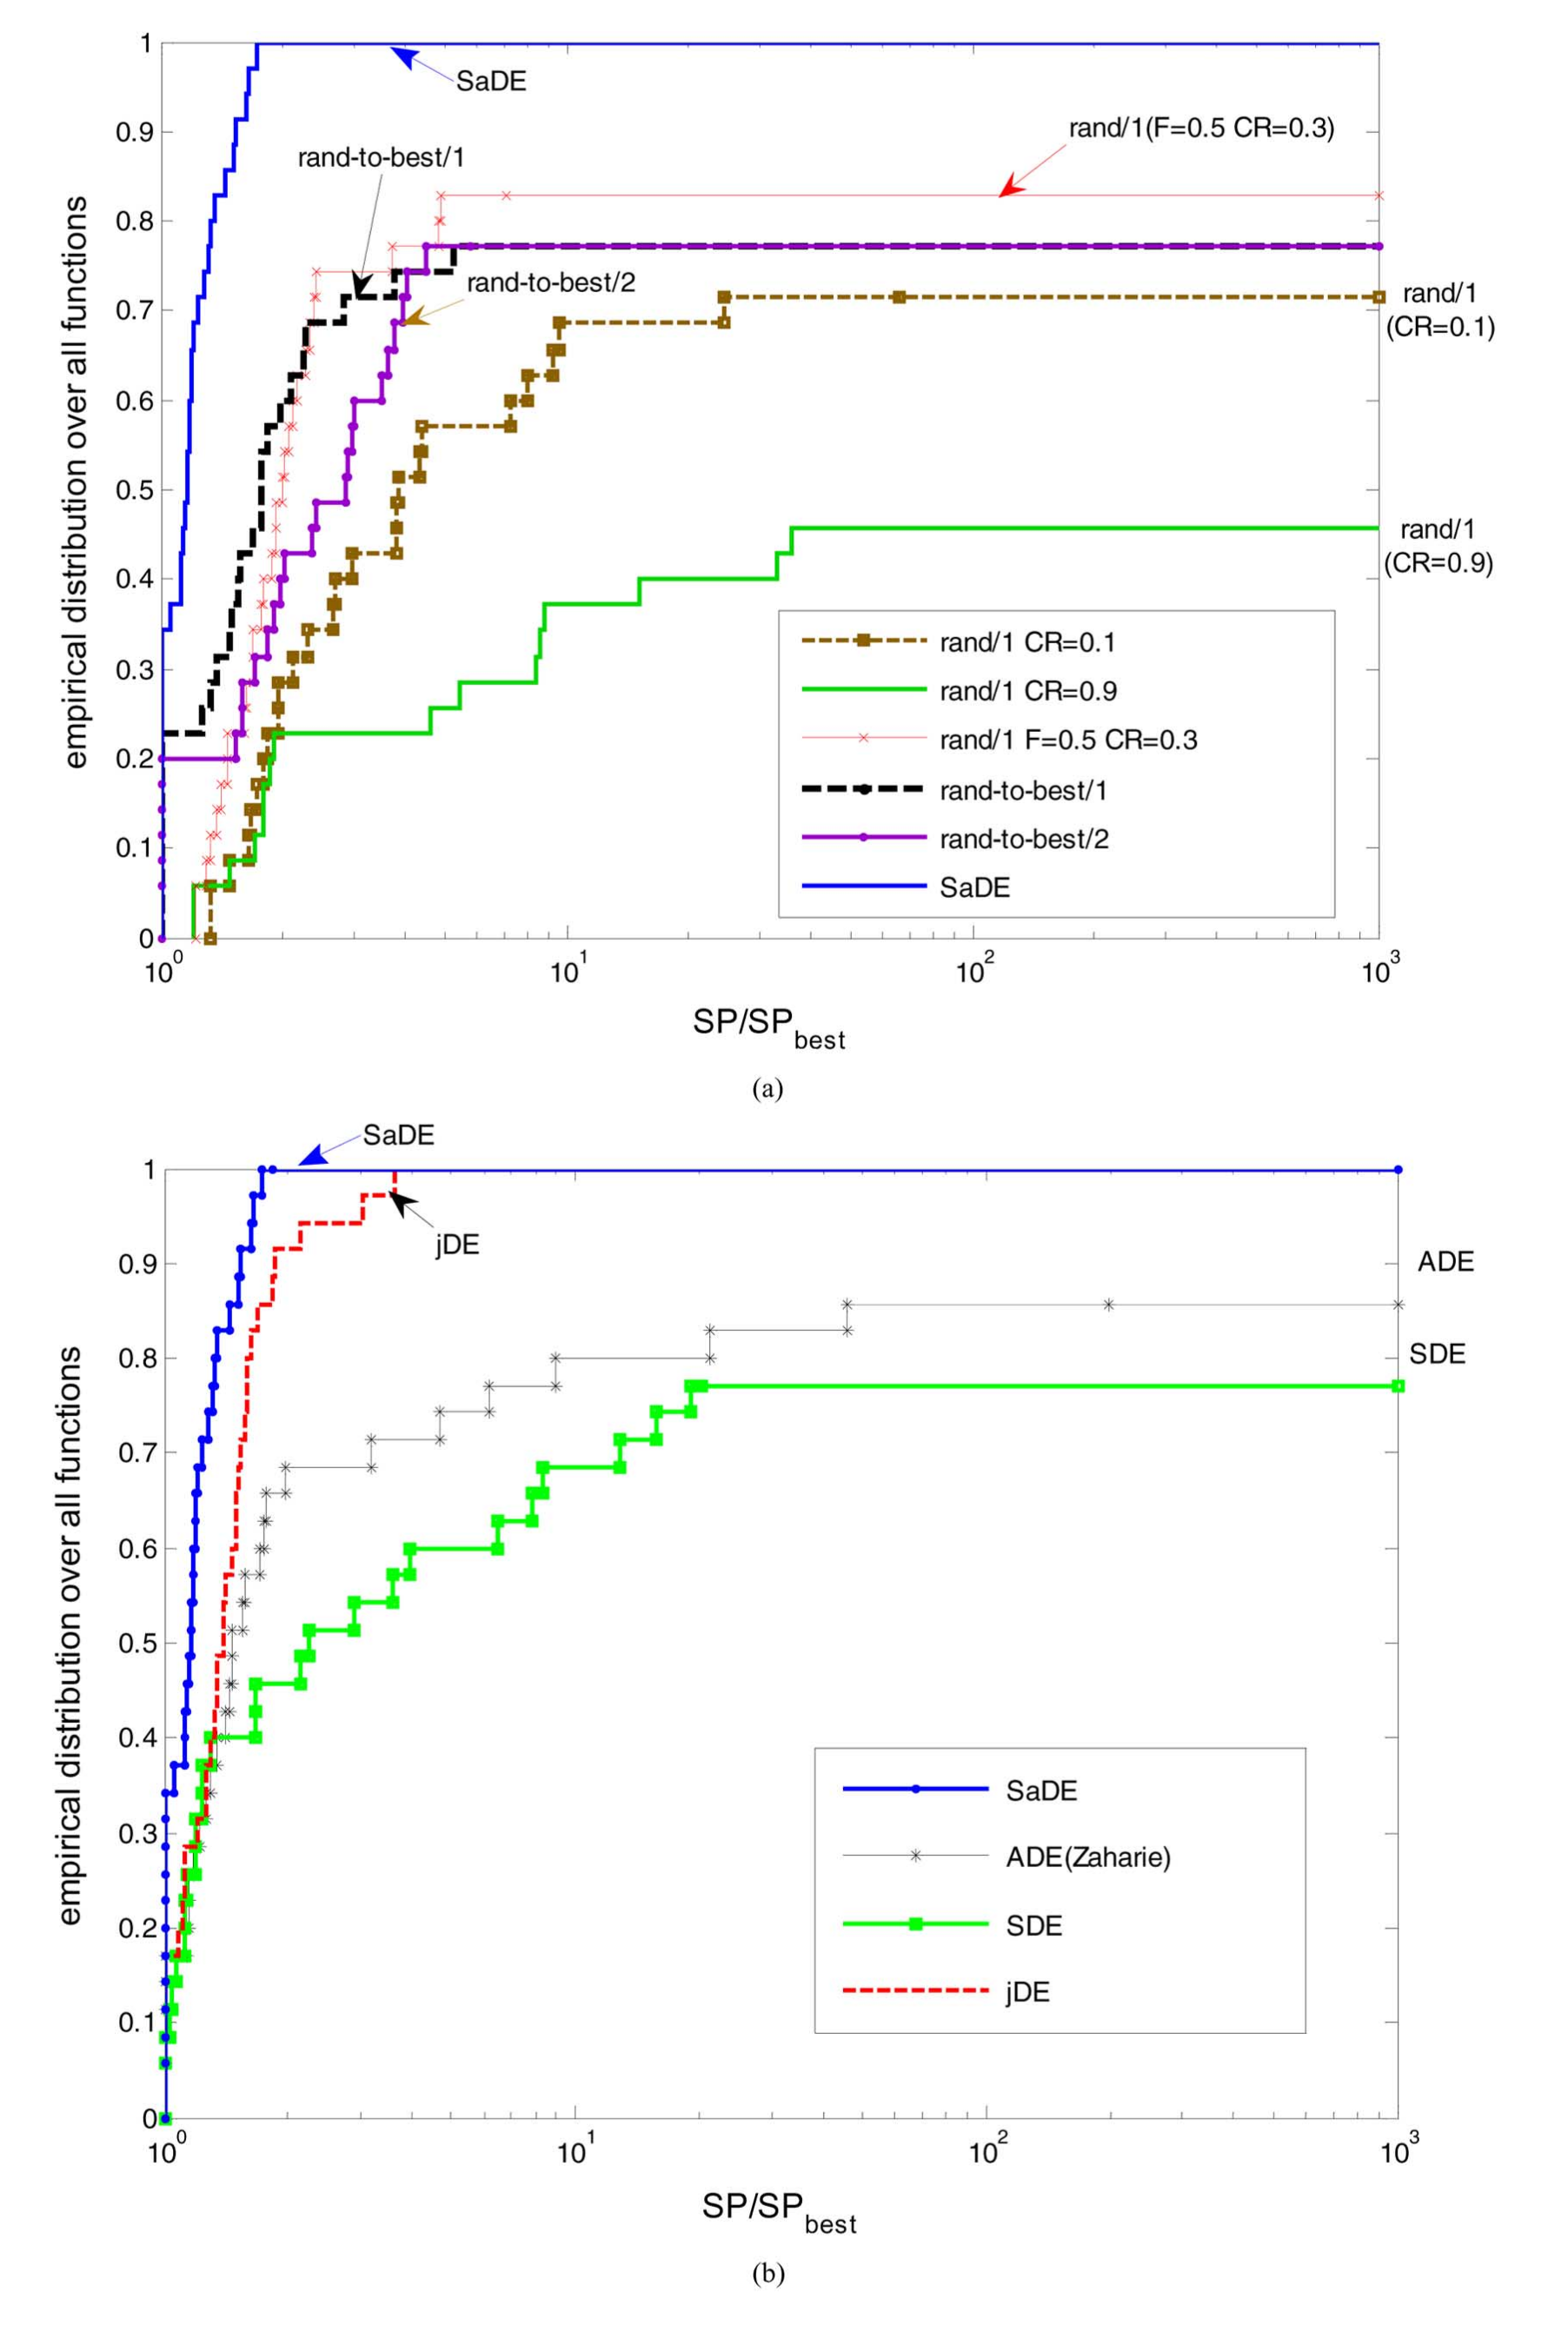
\includegraphics[width=\textwidth]{r5.png}
   \captionof{figure}{توزیع نمونه‌ای کارایی موفقیت برای ۲۶ تابع آزمون}
\label{fig:r5} 
\end{minipage}
}
\end{figure}

در آخر، نتایج این روش با 
\lr{FADE}
نیز مقایسه شده‌است که دلیل آن، آسان بودن حل ابعاد پایین برای هر دو الگوریتم است و نتایج برای مسایل ۵۰ بعدی به صورت خاص برای این دو روش انجام شده‌است. این بررسی در خود مقاله‌ی انتخابی نیز به طور مختصر آورده شده‌است که برتری الگوریتم ارایه‌شده را مشخص می‌کند، اما متاسفانه بررسی الگوریتم \lr{FADE} در مقاله‌ی مورد نظر انجام نگرفته است و از حوصله‌ی این گزارش نیز خارج است.


%\subsection{تحلیل خودتطبیقی \lr{SaDE}} \\ TODO


\newpage
\section{نتیجه‌گیری}

در این مقاله‌، پژوهشگران برای رفع مشکل زمان‌بر بودن جست‌وجو برای یافتن استراتژی مناسب برای تولید بردار آزمایشی در مسایل تکامل تفاضلی و پارامترهای مناسب آن استراتژی، روشی خود تطبیقی ارایه کردند که در آن استراتژی انتخاب بردار آزمایشی و پارامتر
\lr{CR}
متناسب هر استراتژی را در افراد قرار داده‌اند تا تکامل پیدا کند، به این شکل که در طول دوره‌ی یادگیری، نرخ موفقیت هر استراتژی (که در استخر استراتژی ذخیره شده‌اند) و مقادیر مناسب پارامتر یادشده را در حافظه‌هایی نگه‌داری کرده‌اند و پس از اتمام دوره‌ی یادگیری، احتمال انتخاب هر استراتژی و مقادیر مناسب پارامتر بازترکیبی را به‌روز رسانی کرده‌اند. احتمال انتخاب هر استراتژی، متناسب با نرخ تولید بردارهای آزمایشی که موفق به ورود به نسل بعد شده‌اند، به‌روز رسانی شده‌است. مقادیر 
\lr{CR}
نیز با توجه به حساسیت بالای آن، طبق یک تابع توزیع نرمال با واریانس کم تغییر داده شده‌است و برای هر استراتژی در طی دوره‌ی یادگیری ذخیره شده‌است. به‌روز رسانی مقدار این پارامتر به این شکل است که در پایان دوره‌ی یادگیری مقادیر آن برای هر کدام از استراتژی‌ها با میانه‌ی مقادیر این پارامتر در آن دوره، جاگزین می‌شود. انتخاب استراتژی‌هایی با ویژگی‌های متفاوت در استخرِ یاد‌شده، سبب شده‌است این روش در مراحل مختلف تکامل بتواند استراتژی مناسب با مقدار پارامتر مناسب برای آن مرحله را انتخاب کند. آزمایش‌ها بر روی ۲۶ تابع آزمون محبوب و مطرح در تکامل تفاضلی انجام شده‌است و مقایسه‌ها با ۸ روش معمولی و تطبیقی مطرح، انجام شده‌است. به نظر می‌رسد نقطه‌ی قوت اصلی این مقاله در همین مقایسه‌ها و آزمایش‌ها بوده است چرا که با توجه به کارهای انجام‌شده در تکامل تفاضلی که مطالعه شد، تقریبا تمامی جنبه‌های آزمایش‌ها و مقایسه‌ها را مطرح نموده‌است و در انتخاب توابع آزمون نیز کوتاهی نکرده‌است.

 از کارهای آتی این مقاله می‌توان انتظار داشت اندازه‌ی بهینه‌ی استخر استراتژی و معیارهای انتخاب استراتژی‌های استخر را با توجه به ویژگی‌های مساله بررسی کنند. همچنین تطبیق پارامتر 
\lr{F}
و 
\lr{NP}
نیز می‌تواند انجام گیرد. در کل ایده‌ی ساده ولی کار پژوهشی قوی انجام‌شده توسط این پژوهشگران می‌تواند آموزه‌ای برای کارهای آتی در زمینه‌ی تکامل تفاضلی و علاقه‌مندان به تکنیک‌های تکاملی باشد. 


\newpage

\small
%ایجاد «مراجع»
\begin{thebibliography}{99}

\begin{LTRitems}

\resetlatinfont

\bibitem{category}
P. J. Angeline, “Adaptive and self-adaptive evolutionary computation,” In Computational Intelligence: A Dynamic System Perspective, M.Palaniswami, Y. Attikiouzel, R. J. Marks, D. Fogel, and T. Fukuda, Eds. New York: IEEE Press, 1995, pp. 152–161.

\bibitem{adapt-category}
J. E. Smith and T. C. Fogarty, “Operator and parameter adaptation in genetic algorithms,” Soft Comput., vol. 1, no. 2, pp. 81–87, 1997.

\bibitem{DE}
R. Storn and K. V. Price, “Differential evolution-A simple and efficient heuristic for global optimization over continuous Spaces,” J. Global Optim., vol. 11, pp. 341–359, 1997.

\bibitem{Sade}
A. K. Qin, V. L. Huang, and P. N. Suganthan “Differential Evolution Algorithm With Strategy
Adaptation for Global Numerical Optimization,” Evolutionary Computation, IEEE Transactions on, vol. 13, no. 2, 398-417, 2009.

\bibitem{demon1}
K. Price, R. Storn and J. Lampinen, “Differential Evolution — A Practical Approach to Global Optimization,” Berlin, Germany: Springer-Verlag, 2005.

\bibitem{demon2}
J. Lampinen and I. Zelinka, “On stagnation of the differential evolution algorithm,” In Proc. 6th Int. Mendel Conf. Soft Comput., P. Osmera, Ed., pp. 76–83, 2002.

\bibitem{demon3}
R. Gämperle, S. D. Müller, and P. Koumoutsakos, “A parameter study for differential evolution,” In Advances in Intelligent Systems, Fuzzy Systems, Evolutionary Computation, A. Grmela and N. E. Mastorakis, Eds. Interlaken, Switzerland: WSEAS Press, pp. 293–298, 2002.

\bibitem{demon4}
D. Zaharie, “Control of population diversity and adaptation in differential evolution algorithms,” In Proc. Mendel 9th Int. Conf. Soft Comput., R. Matousek and P. Osmera, Eds., Brno, Czech Republic, pp. 41–46, 2003.

\bibitem{demon5}
S. Das, A. Konar, and U. K. Chakraborty, “Two improved differential evolution schemes for faster global search,” In ACM-SIGEVO Proc. Genetic Evolut. Comput. Conf., Washington, DC, pp. 991–998, 2005.

\bibitem{pso}
J. Kennedy, and E. Russell, “Particle swarm optimization,” In Proceedings of 1995 IEEE International Conference on Neural Networks, pp. 1942-1948, 1995.

\bibitem{pso-tviw}
Y. Shi, and R. C. Eberhart, “Empirical study of particle swarm optimization.” In Evolutionary Computation, CEC 99, Proceedings of the 1999 Congress on, IEEE, vol. 3, pp. 1945-1950, 1999.

\bibitem{pso-randiw}
Y. Shi, and R. C. Eberhart, “Particle swarm optimization: developments, applications and resources.” In Evolutionary Computation, Proceedings of the 2001 Congress on, IEEE, vol. 1, pp. 81-86, 2001.

\bibitem{15}
R. Storn and K. Price, “Differential evolution-a simple and efficient adaptive scheme for global optimization over continuous spaces,” Berkeley: ICSI, 1995. Available: http://http.icsi.berkeley.edu/$\sim$storn/litera.html

\bibitem{20}
K. V. Price, “An introduction to differential evolution,” In New Ideas in Optimization, D. Corne, M. Dorigo, and F. Glover, Eds. London, U.K.: McGraw-Hill, pp. 79–108, 1999.

\bibitem{21}
J. Rönkkönen, S. Kukkonen, and K. V. Price, “Real parameter optimization with differential evolution,” In Proc. IEEE Congr. Evolut. Comput., Edinburgh, Scotland, pp. 506–513, 2005.

\bibitem{ASA}
L. Ingber, “Simulated annealing: Practice versus theory.” Mathematical and computer modelling, vol.18, no. 11, pp. 29-57, 1993.


\bibitem{ANM}
W. H. Press,  S. A. Teukolsky, B. P. Flannery, and W. T. Vetterling, “Numerical recipes in C,” Cambridge: Cambridge University, pp. 545-555, 1992.

\bibitem{cma-es}
Nikolaus Hansen, and A. Ostermeier, “Convergence Properties of Evolution Strategies with the Derandomized Covariance Matrix Adaptation: The $(\mu/\mu\_I, \lambda)$-ES,” In Proceedings of the 5th European Congress on Intelligent Techniques and Soft Computing (EUFIT’97), pp. 650-654, 1997.

\bibitem{18}
J. Liu, and J. Lampinen, “A fuzzy adaptive differential evolution algorithm,” Soft Comput., vol. 9, no. 6, pp. 448–462, 2005.

\bibitem{25}
D. Zaharie, and D. Petcu, “Adaptive pareto differential evolution and its parallelization,” in Proc. 5th Int. Conf. Parallel Process. Appl. Math., Czestochowa, Poland, pp. 261–268, 2003.

\bibitem{26}
H. A. Abbass, “The self-adaptive Pareto differential evolution algorithm,” in Proc. Congr. Evolut. Comput., Honolulu, HI, pp. 831–836, 2002.

\bibitem{oldwork}
A. K. Qin, and P. N. Suganthan, “Self-adaptive differential evolution algorithm for numerical optimization,” in Proc. IEEE Congr. Evolut.
Comput., Edinburgh, Scotland, pp. 1785–1791, 2005.

\bibitem{27}
M. G. H. Omran, A. Salman, and A. P. Engelbrecht, “Self-adaptive differential evolution,” in Lecture Notes in Artificial Intelligence. Berlin, Germany: Springer-Verlag, pp. 192–199, 2005.

\bibitem{22}
J. Teo, “Exploring dynamic self-adaptive populations in differential evolution,” Soft Comput., vol. 10, no. 8, pp. 637–686, 2006.

\bibitem{28}
J. Brest, S. Greiner, B. Boskovic, M. Mernik, and V. Zumer, “Self-adapting control parameters in differential evolution: A comparative study on numerical benchmark problems,” IEEE Trans. Evolut. Comput., vol. 10, no. 6, pp. 646–657, 2006.

\bibitem{11}
R. Storn, “On the usage of differential evolution for function optimization,” in Proc. Biennial Conf. North Amer. Fuzzy Inf. Process. Soc., Berkeley, CA, pp. 519-523, 1996.

\bibitem{selection}
J. E. Baker, “Reducing bias and inefficiency in the selection algorithm,” In Proc. 2nd Int. Conf. Genetic Algorithms, Cambridge, pp. 14–21, 1987.

\bibitem{32-cf}
J. J. Liang, P. N. Suganthan, and K. Deb, “Novel composition test functions for numerical global optimization,” In Proc. IEEE Swarm Intell. Symp., Pasadena, CA, pp. 68–75, 2005.

\bibitem{36}
N. Hansen, “Compilation of results on the 2005 CEC benchmark function set,” May 4, 2006 [Online]. Available: http://www.ntu.edu.sg/home/epnsugan/index\_files/CEC-05/compareresults.pdf

\end{LTRitems}

\end{thebibliography}

\end{document} 
